\FloatBarrier{}
\section{Comparison}
Now we compare the two methods.
\subsection{Single element test: $\nu$ sweep}

We begin with a single element test. First on a third-order HEX8 element of dimension $L\times{}L\times L{}$. The boundary conditions are the following,

\begin{align*}
    U_y^{(i)} &= 0.2\,(t/T)\,X_0^{(i)} \quad \text{for each node } i \in \{Y = L\}, \\
    U_y &= 0 \quad \text{on } \{Y = 0\}, \\
    U_x &= 0 \quad \text{on } \{X = 0\}, \\
    U_z &= 0 \quad \text{on } \{Z = 0, Z = L\}.\\
\end{align*}

The boundary condition at $Y=L$ is applied per node, and leads the $\nabla U$ field to vary per QP. As such, $J$ and $F$ vary per QP, allow for F-bar to switch on. Figure~\ref{fig:hex8} shows the initial and final configurations of the HEX8 element.

\begin{figure}
    \centering
    \begin{subfigure}{0.45\textwidth}
        \centering
        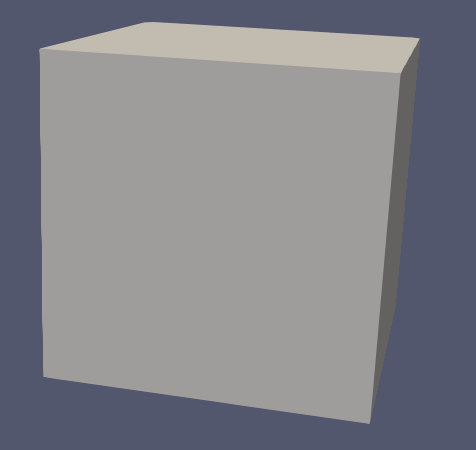
\includegraphics[width=0.5\textwidth]{pictures/HEX8_initial.png}
    \end{subfigure}
    \begin{subfigure}{0.45\textwidth}
        \centering
        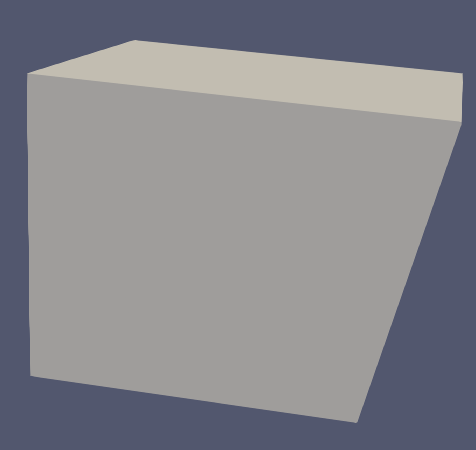
\includegraphics[width=0.5\textwidth]{pictures/HEX8_final.png}
    \end{subfigure}
    \caption{Initial~(left) and final~(right) configurations of the HEX8 element.}
    \label{fig:hex8}
\end{figure}

Several cases are considered:
\begin{itemize}
    \item Quasi-static + Elasticity
    \item Dynamics + Elasticity
    \item Quasi-static + Elasticity + Plasticity
    \item Dynamics + Elasticity + Plasticity
\end{itemize}

The difference between the uncorrected and volumetric Cauchy stress is used as the metric for the amount of correction present:
\begin{equation}
    P_{\text{diff}} = K(\bar{J}-J),
\end{equation}
where $K$ is the bulk modulus, J is the Jacobian, and $\bar{J}$ is the volume averaged Jacobian. The relative error is calculated as
\begin{equation}
    \left[\frac{\int_{\Omega_1}\psi^e_1-\int_{\Omega_0}\psi^e_0}{\int_{\Omega_0}\psi^e_0}\right]_{t=t_r+\Delta t},
\end{equation}
where $\psi^e$ is the elastic energy and $t_r$ is the time of recovery. The 0th simulation is ran for an extra step into order to compute fields at $t_r+\Delta t$. The restarted simulation uses the field data at $t=t_r$.

Figure~\ref{fig:se_strength_comparison_quasi_elastic} compares the initial relative error for the quasi-static elastic case. Clearly, method \#2 performs better than method \#1, with the error of method \#1 increasing with the amount of pressure correction present. The error of method \#2 is on the order of machine precision. Figure~\ref{fig:se_energy_elastic_qs} reflects this pattern through the plotting of the total elastic energy in the sample over time. Method \#1 shows a clear deviation in the total elastic at the restart, even if small. No visible in the restart is seen when using method \#2.

Figure~\ref{fig:se_strength_comparison_elastic} compares the initial relative error for the dynamic elastic case. It is clear that method \#2 performs better than method \#1, but the error is no longer on the order of machine precision, and clearly increases as the amount of correction present increases.

% Include in main.tex with: \input{figures/bc_strength_comparison_quasi_elastic}
% Requires in preamble: \usepackage{pgfplots}, \pgfplotsset{compat=1.18}
%                       \usepgfplotslibrary{groupplots}
\begin{figure}[htbp]
\centering
\begin{tikzpicture}
\begin{groupplot}[
    group style={
        group size=2 by 1,
        horizontal sep=1.8cm,
    },
    width=0.42\textwidth,
    height=0.42\textwidth,
    grid=major,
    grid style={gray!25},
    tick align=outside,
    xlabel={Max F-bar pressure correction (ref)},
    nodes near coords,
    nodes near coords style={font=\small, anchor=south west},
    point meta=explicit symbolic,
]

%% --- Left panel: method 1 (old) ---
\nextgroupplot[
    title={Method \#1},
    ylabel={Relative error at target},
    ymax=0.04,
    ymin=0
]
\addplot[only marks, mark=*, mark size=3pt, red] table[
    col sep=comma,
    x=fbar_pressure_correction_max_ref,
    y=rel_err_target,
    meta=nu
]{/home/det12/projects/latex/fbar_writeup/data/single_element/elastic_qs/error/nu_sweep_results_old.csv};

%% --- Right panel: method 2 (new) ---
\nextgroupplot[
    title={Method \#2},
    ylabel={Relative error at target},
    yticklabel pos=right,
    ymax=0.04,
    ymin=0
]
\addplot[only marks, mark=*, mark size=3pt, blue] table[
    col sep=comma,
    x=fbar_pressure_correction_max_ref,
    y=rel_err_target,
    meta=nu
]{/home/det12/projects/latex/fbar_writeup/data/single_element/elastic_qs/error/nu_sweep_results_new.csv};

\end{groupplot}
\end{tikzpicture}
\caption{$\nu$ sweep, quasi-static-elastic case: Relative error at target vs.\ maximum F-bar pressure correction for method \#1 (left) and method \#2 (right), with the boundary-condition case labelled at each point.}
\label{fig:bc_strength_comparison_quasi_elastic}
\end{figure}

% Include with: % Include with: % Include with: \input{figures/single_element/single_element_energy_elastic_quasi}
\begin{figure}[htbp]
\centering
\begin{tikzpicture}
\begin{groupplot}[
    group style={group size=2 by 1, horizontal sep=1.6cm},
    width=0.46\textwidth,
    height=0.46\textwidth,
    grid=major, grid style={gray!25},
    tick align=outside,
    xlabel={Time},
    ylabel={$\displaystyle\int_\Omega \psi_e \, dV$},
    xmin=0, xmax=1.25,
    legend style={font=\scriptsize, cells={anchor=west}},
    legend pos=north west,
]

%% --- Left: Method #1 (old) ---
\nextgroupplot[title={Method \#1}]
\addplot[blue,             line width=2pt, solid] table[col sep=comma, x=time, y=psie_active_int]{data/single_element/elastic_qs/old/pull_test_out_nu_0p30_old.csv};   \addlegendentry{$\nu=0.30$}
\addplot[violet,           line width=2pt, solid] table[col sep=comma, x=time, y=psie_active_int]{data/single_element/elastic_qs/old/pull_test_out_nu_0p499_old.csv};  \addlegendentry{$\nu=0.499$}
\addplot[red,            thick, dashed, restrict x to domain=1.0001:100] table[col sep=comma, x=time, y=psie_active_int]{data/single_element/elastic_qs/old/pull_test_restart_out_nu_0p30_old.csv};
\addplot[orange,         thick, dashed, restrict x to domain=1.0001:100] table[col sep=comma, x=time, y=psie_active_int]{data/single_element/elastic_qs/old/pull_test_restart_out_nu_0p499_old.csv};
\draw[black!50, dashed] (axis cs:1.0,0) -- (axis cs:1.0,0.012);
\node[above, font=\tiny, rotate=90] at (axis cs:0.97,0.002) {restart};

%% --- Right: Method #2 (new) ---
\nextgroupplot[title={Method \#2}, yticklabel pos=right]
\addplot[blue,             line width=2pt, solid] table[col sep=comma, x=time, y=psie_active_int]{data/single_element/elastic_qs/new/pull_test_out_nu_0p30_new.csv};
\addplot[violet,           line width=2pt, solid] table[col sep=comma, x=time, y=psie_active_int]{data/single_element/elastic_qs/new/pull_test_out_nu_0p499_new.csv};
\addplot[red,            thick, dashed, restrict x to domain=1.0001:100] table[col sep=comma, x=time, y=psie_active_int]{data/single_element/elastic_qs/new/pull_test_restart_out_nu_0p30_new.csv};
\addplot[orange,         thick, dashed, restrict x to domain=1.0001:100] table[col sep=comma, x=time, y=psie_active_int]{data/single_element/elastic_qs/new/pull_test_restart_out_nu_0p499_new.csv};
\draw[black!50, dashed] (axis cs:1.0,0) -- (axis cs:1.0,0.012);
\node[above, font=\tiny, rotate=90] at (axis cs:0.97,0.002) {restart};

\end{groupplot}
\end{tikzpicture}
\caption{Single element, quasi-static-elastic: Integrated elastic energy vs.\ time for method \#1 (left) and method \#2 (right). Solid lines: reference. Dashed lines: restart (red: $\nu=0.30$, orange: $\nu=0.499$). Legend in left panel applies to both.}
\label{fig:se_energy_elastic_qs}
\end{figure}

\begin{figure}[htbp]
\centering
\begin{tikzpicture}
\begin{groupplot}[
    group style={group size=2 by 1, horizontal sep=1.6cm},
    width=0.46\textwidth,
    height=0.46\textwidth,
    grid=major, grid style={gray!25},
    tick align=outside,
    xlabel={Time},
    ylabel={$\displaystyle\int_\Omega \psi_e \, dV$},
    xmin=0, xmax=1.25,
    legend style={font=\scriptsize, cells={anchor=west}},
    legend pos=north west,
]

%% --- Left: Method #1 (old) ---
\nextgroupplot[title={Method \#1}]
\addplot[blue,             line width=2pt, solid] table[col sep=comma, x=time, y=psie_active_int]{data/single_element/elastic_qs/old/pull_test_out_nu_0p30_old.csv};   \addlegendentry{$\nu=0.30$}
\addplot[violet,           line width=2pt, solid] table[col sep=comma, x=time, y=psie_active_int]{data/single_element/elastic_qs/old/pull_test_out_nu_0p499_old.csv};  \addlegendentry{$\nu=0.499$}
\addplot[red,            thick, dashed, restrict x to domain=1.0001:100] table[col sep=comma, x=time, y=psie_active_int]{data/single_element/elastic_qs/old/pull_test_restart_out_nu_0p30_old.csv};
\addplot[orange,         thick, dashed, restrict x to domain=1.0001:100] table[col sep=comma, x=time, y=psie_active_int]{data/single_element/elastic_qs/old/pull_test_restart_out_nu_0p499_old.csv};
\draw[black!50, dashed] (axis cs:1.0,0) -- (axis cs:1.0,0.012);
\node[above, font=\tiny, rotate=90] at (axis cs:0.97,0.002) {restart};

%% --- Right: Method #2 (new) ---
\nextgroupplot[title={Method \#2}, yticklabel pos=right]
\addplot[blue,             line width=2pt, solid] table[col sep=comma, x=time, y=psie_active_int]{data/single_element/elastic_qs/new/pull_test_out_nu_0p30_new.csv};
\addplot[violet,           line width=2pt, solid] table[col sep=comma, x=time, y=psie_active_int]{data/single_element/elastic_qs/new/pull_test_out_nu_0p499_new.csv};
\addplot[red,            thick, dashed, restrict x to domain=1.0001:100] table[col sep=comma, x=time, y=psie_active_int]{data/single_element/elastic_qs/new/pull_test_restart_out_nu_0p30_new.csv};
\addplot[orange,         thick, dashed, restrict x to domain=1.0001:100] table[col sep=comma, x=time, y=psie_active_int]{data/single_element/elastic_qs/new/pull_test_restart_out_nu_0p499_new.csv};
\draw[black!50, dashed] (axis cs:1.0,0) -- (axis cs:1.0,0.012);
\node[above, font=\tiny, rotate=90] at (axis cs:0.97,0.002) {restart};

\end{groupplot}
\end{tikzpicture}
\caption{Single element, quasi-static-elastic: Integrated elastic energy vs.\ time for method \#1 (left) and method \#2 (right). Solid lines: reference. Dashed lines: restart (red: $\nu=0.30$, orange: $\nu=0.499$). Legend in left panel applies to both.}
\label{fig:se_energy_elastic_qs}
\end{figure}

\begin{figure}[htbp]
\centering
\begin{tikzpicture}
\begin{groupplot}[
    group style={group size=2 by 1, horizontal sep=1.6cm},
    width=0.46\textwidth,
    height=0.46\textwidth,
    grid=major, grid style={gray!25},
    tick align=outside,
    xlabel={Time},
    ylabel={$\displaystyle\int_\Omega \psi_e \, dV$},
    xmin=0, xmax=1.25,
    legend style={font=\scriptsize, cells={anchor=west}},
    legend pos=north west,
]

%% --- Left: Method #1 (old) ---
\nextgroupplot[title={Method \#1}]
\addplot[blue,             line width=2pt, solid] table[col sep=comma, x=time, y=psie_active_int]{data/single_element/elastic_qs/old/pull_test_out_nu_0p30_old.csv};   \addlegendentry{$\nu=0.30$}
\addplot[violet,           line width=2pt, solid] table[col sep=comma, x=time, y=psie_active_int]{data/single_element/elastic_qs/old/pull_test_out_nu_0p499_old.csv};  \addlegendentry{$\nu=0.499$}
\addplot[red,            thick, dashed, restrict x to domain=1.0001:100] table[col sep=comma, x=time, y=psie_active_int]{data/single_element/elastic_qs/old/pull_test_restart_out_nu_0p30_old.csv};
\addplot[orange,         thick, dashed, restrict x to domain=1.0001:100] table[col sep=comma, x=time, y=psie_active_int]{data/single_element/elastic_qs/old/pull_test_restart_out_nu_0p499_old.csv};
\draw[black!50, dashed] (axis cs:1.0,0) -- (axis cs:1.0,0.012);
\node[above, font=\tiny, rotate=90] at (axis cs:0.97,0.002) {restart};

%% --- Right: Method #2 (new) ---
\nextgroupplot[title={Method \#2}, yticklabel pos=right]
\addplot[blue,             line width=2pt, solid] table[col sep=comma, x=time, y=psie_active_int]{data/single_element/elastic_qs/new/pull_test_out_nu_0p30_new.csv};
\addplot[violet,           line width=2pt, solid] table[col sep=comma, x=time, y=psie_active_int]{data/single_element/elastic_qs/new/pull_test_out_nu_0p499_new.csv};
\addplot[red,            thick, dashed, restrict x to domain=1.0001:100] table[col sep=comma, x=time, y=psie_active_int]{data/single_element/elastic_qs/new/pull_test_restart_out_nu_0p30_new.csv};
\addplot[orange,         thick, dashed, restrict x to domain=1.0001:100] table[col sep=comma, x=time, y=psie_active_int]{data/single_element/elastic_qs/new/pull_test_restart_out_nu_0p499_new.csv};
\draw[black!50, dashed] (axis cs:1.0,0) -- (axis cs:1.0,0.012);
\node[above, font=\tiny, rotate=90] at (axis cs:0.97,0.002) {restart};

\end{groupplot}
\end{tikzpicture}
\caption{Single element, quasi-static-elastic: Integrated elastic energy vs.\ time for method \#1 (left) and method \#2 (right). Solid lines: reference. Dashed lines: restart (red: $\nu=0.30$, orange: $\nu=0.499$). Legend in left panel applies to both.}
\label{fig:se_energy_elastic_qs}
\end{figure}


\input{figures/single_element/single_element_error_elastic}
\input{figures/single_element/single_element_energy_elastic}

% Include in main.tex with: % Include in main.tex with: % Include in main.tex with: \input{figures/single_element/single_element_error_plastic_quasi}
% Requires in preamble: \usepackage{pgfplots}, \pgfplotsset{compat=1.18}
%                       \usepgfplotslibrary{groupplots}
\begin{figure}[htbp]
\centering
\begin{tikzpicture}
\begin{groupplot}[
    group style={
        group size=2 by 1,
        horizontal sep=1.8cm,
    },
    width=0.42\textwidth,
    height=0.42\textwidth,
    grid=major,
    grid style={gray!25},
    tick align=outside,
    xlabel={Max F-bar pressure correction (ref)},
    xmode=log,
    ymode=log,
    nodes near coords,
    nodes near coords style={font=\small, anchor=south west},
    point meta=explicit symbolic,
]

%% --- Left panel: method 1 (old) ---
\nextgroupplot[
    title={Method \#1},
    ylabel={Relative error at first step},
    % ymax=0.01,
]
\addplot[only marks, mark=*, mark size=3pt, red] table[
    col sep=comma,
    x=fbar_pressure_correction_max_ref,
    y=rel_err_first,
    meta=nu
]{data/single_element/plastic_qs/error/nu_sweep_results_old.csv};

\addplot[only marks, mark=*, mark size=3pt, blue] table[
    col sep=comma,
    x=fbar_pressure_correction_max_ref,
    y=rel_err_first,
    meta=nu
]{data/single_element/plastic_qs/error/nu_sweep_results_new.csv};

%% --- Right panel: method 2 (new) ---
\nextgroupplot[
    title={Method \#2},
    ylabel={Relative error at first step},
    yticklabel pos=right,
    ymax=0.01,
]
\addplot[only marks, mark=*, mark size=3pt, blue] table[
    col sep=comma,
    x=fbar_pressure_correction_max_ref,
    y=rel_err_first,
    meta=nu
]{data/single_element/plastic_qs/error/nu_sweep_results_new.csv};

\end{groupplot}
\end{tikzpicture}
\caption{$\nu$ sweep, quasi-static-plastic case: Relative error at target vs.\ maximum F-bar pressure correction for method \#1 (left) and method \#2 (right), with Poisson's ratio labelled at each point.}
\label{fig:bc_strength_comparison_plastic_quasi}
\end{figure}

% Requires in preamble: \usepackage{pgfplots}, \pgfplotsset{compat=1.18}
%                       \usepgfplotslibrary{groupplots}
\begin{figure}[htbp]
\centering
\begin{tikzpicture}
\begin{groupplot}[
    group style={
        group size=2 by 1,
        horizontal sep=1.8cm,
    },
    width=0.42\textwidth,
    height=0.42\textwidth,
    grid=major,
    grid style={gray!25},
    tick align=outside,
    xlabel={Max F-bar pressure correction (ref)},
    xmode=log,
    ymode=log,
    nodes near coords,
    nodes near coords style={font=\small, anchor=south west},
    point meta=explicit symbolic,
]

%% --- Left panel: method 1 (old) ---
\nextgroupplot[
    title={Method \#1},
    ylabel={Relative error at first step},
    % ymax=0.01,
]
\addplot[only marks, mark=*, mark size=3pt, red] table[
    col sep=comma,
    x=fbar_pressure_correction_max_ref,
    y=rel_err_first,
    meta=nu
]{data/single_element/plastic_qs/error/nu_sweep_results_old.csv};

\addplot[only marks, mark=*, mark size=3pt, blue] table[
    col sep=comma,
    x=fbar_pressure_correction_max_ref,
    y=rel_err_first,
    meta=nu
]{data/single_element/plastic_qs/error/nu_sweep_results_new.csv};

%% --- Right panel: method 2 (new) ---
\nextgroupplot[
    title={Method \#2},
    ylabel={Relative error at first step},
    yticklabel pos=right,
    ymax=0.01,
]
\addplot[only marks, mark=*, mark size=3pt, blue] table[
    col sep=comma,
    x=fbar_pressure_correction_max_ref,
    y=rel_err_first,
    meta=nu
]{data/single_element/plastic_qs/error/nu_sweep_results_new.csv};

\end{groupplot}
\end{tikzpicture}
\caption{$\nu$ sweep, quasi-static-plastic case: Relative error at target vs.\ maximum F-bar pressure correction for method \#1 (left) and method \#2 (right), with Poisson's ratio labelled at each point.}
\label{fig:bc_strength_comparison_plastic_quasi}
\end{figure}

% Requires in preamble: \usepackage{pgfplots}, \pgfplotsset{compat=1.18}
%                       \usepgfplotslibrary{groupplots}
\begin{figure}[htbp]
\centering
\begin{tikzpicture}
\begin{groupplot}[
    group style={
        group size=2 by 1,
        horizontal sep=1.8cm,
    },
    width=0.42\textwidth,
    height=0.42\textwidth,
    grid=major,
    grid style={gray!25},
    tick align=outside,
    xlabel={Max F-bar pressure correction (ref)},
    xmode=log,
    ymode=log,
    nodes near coords,
    nodes near coords style={font=\small, anchor=south west},
    point meta=explicit symbolic,
]

%% --- Left panel: method 1 (old) ---
\nextgroupplot[
    title={Method \#1},
    ylabel={Relative error at first step},
    % ymax=0.01,
]
\addplot[only marks, mark=*, mark size=3pt, red] table[
    col sep=comma,
    x=fbar_pressure_correction_max_ref,
    y=rel_err_first,
    meta=nu
]{data/single_element/plastic_qs/error/nu_sweep_results_old.csv};

\addplot[only marks, mark=*, mark size=3pt, blue] table[
    col sep=comma,
    x=fbar_pressure_correction_max_ref,
    y=rel_err_first,
    meta=nu
]{data/single_element/plastic_qs/error/nu_sweep_results_new.csv};

%% --- Right panel: method 2 (new) ---
\nextgroupplot[
    title={Method \#2},
    ylabel={Relative error at first step},
    yticklabel pos=right,
    ymax=0.01,
]
\addplot[only marks, mark=*, mark size=3pt, blue] table[
    col sep=comma,
    x=fbar_pressure_correction_max_ref,
    y=rel_err_first,
    meta=nu
]{data/single_element/plastic_qs/error/nu_sweep_results_new.csv};

\end{groupplot}
\end{tikzpicture}
\caption{$\nu$ sweep, quasi-static-plastic case: Relative error at target vs.\ maximum F-bar pressure correction for method \#1 (left) and method \#2 (right), with Poisson's ratio labelled at each point.}
\label{fig:bc_strength_comparison_plastic_quasi}
\end{figure}

\input{figures/single_element/single_element_energy_plastic_quasi}

\input{figures/single_element/single_element_error_plastic}
\input{figures/single_element/single_element_energy_plastic}

\FloatBarrier{}



\subsection{Multi-element test}
Figure~\ref{fig:domain} shows the domain, which an $L\times{}L\times L{}$ cube consisting of TET10 elements, where $L=3$. The elasticity model compressible Neo-Hookean hyper-elasticity and the plasticity model is $J_2$ plasticity with Johnson-Cook hardening/softening.

\begin{figure}[htb]
    \centering
    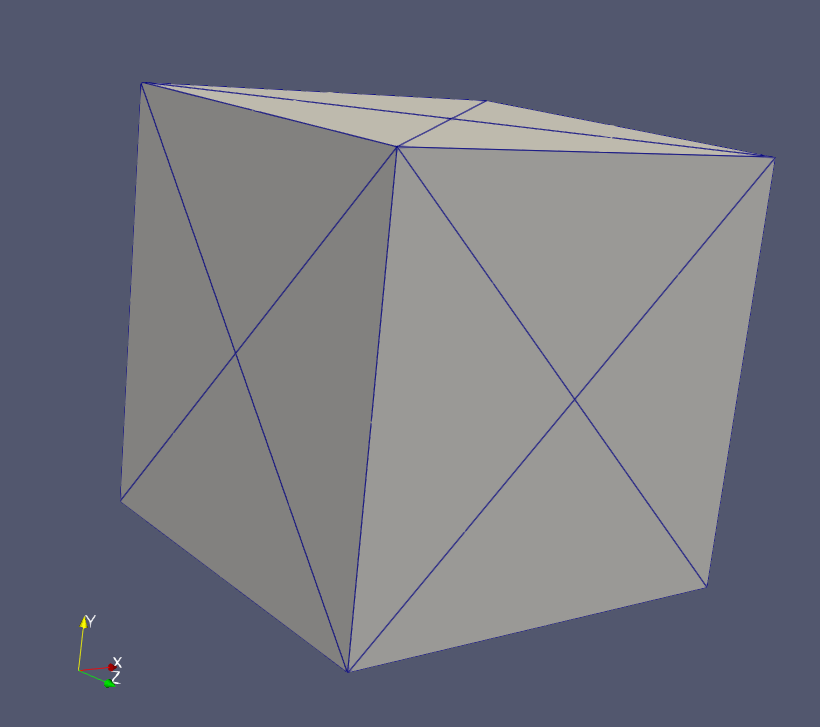
\includegraphics[width=0.25\textwidth]{pictures/mesh.png}
    \caption{Domain.}
    \label{fig:domain}
\end{figure}

The following boundary conditions are applied to force regions of artificial stiffness,

\begin{align*}
    U_y &= t \quad \text{on } \{Y = L\}, \\
    U_y &= 0 \quad \text{on } \{Y = 0\}, \\
    U_x &= 0 \quad \text{on } \{X = 0, Y = L\}, \\
    U_z &= 0 \quad \text{on } \{Z = 0, Z = L\}.\\
\end{align*}

The boundary conditions lead a single free surface at $X=L$. The following simulations modify the amount of applied correction varying the poissons ratio, \\$\nu = \{0.3,0.4.0.45,0.48,0.49,0.459\}$, with the most correction occurring at $\nu=0.459$. The difference between the uncorrected and volumetric Cauchy stress is used as the metric for how much correction occurs:
\begin{equation}
    P_{\text{diff}} = K(\bar{J}-J),
\end{equation}
where $K$ is the bulk modulus, J is the Jacobian, and $\bar{J}$ is the volume averaged Jacobian. The relative error is calculated as
\begin{equation}
    \left[\frac{\int_{\Omega_1}\psi^e_1-\int_{\Omega_0}\psi^e_0}{\int_{\Omega_0}\psi^e_0}\right]_{t=t_r+\Delta t},
\end{equation}
where $\psi^e$ is the elastic energy and $t_r$ is the time of recovery. The 0th simulation is ran for an extra step into order to compute fields at $t_r+\Delta t$. The restarted simulation uses the field data at $t=t_r$.

Several different scenarios are considered for the comparison:
\begin{itemize}
    \item Quasi-static + elastic: Figures~\ref{fig:fbar_strength_comparison_elastic_quasi},~\ref{fig:elastic_energy_quasi_elastic}
    \item Dynamic + elastic: Figures:~\ref{fig:fbar_strength_comparison_elastic},\ref{fig:elastic_energy_dynamic_elastic}
    \item Quasi-static + elastic + plastic: Figures~\ref{fig:fbar_strength_comparison_quasi},\ref{fig:elastic_energy_quasi_elastic}
    \item Dynamic + elastic + plastic: Figures~\ref{fig:fbar_strength_comparison},\ref{fig:fbar_strength_comparison}
\end{itemize}

% % Include in main.tex with: % Include in main.tex with: % Include in main.tex with: \input{figures/fbar_comparison}
% Requires in preamble: \usepackage{pgfplots}, \pgfplotsset{compat=1.18}
%                       \usepgfplotslibrary{groupplots}
\begin{figure}[htbp]
\centering
\begin{tikzpicture}
\begin{groupplot}[
    group style={
        group size=2 by 1,
        horizontal sep=1.5cm,
    },
    width=0.42\textwidth,
    height=0.42\textwidth,
    grid=major,
    grid style={gray!25},
    tick align=outside,
    xmin=0, xmax=2.5,
    legend style={font=\small, cells={anchor=west}},
    legend pos=north west,
]

%% --- Left panel: integrated effective plastic strain ---
\nextgroupplot[
    ylabel={$\displaystyle\int_\Omega \varepsilon^p \, dV$},
    xlabel={Time},
]

% Reference runs (solid)
\addplot[blue,   thick, solid]
    table[col sep=comma, x=time, y=ep_int]{data/nu_sweep/parallel/reference_fbar_out_1.csv};
\addlegendentry{Ref $n=1$}

\addplot[red,    thick, solid]
    table[col sep=comma, x=time, y=ep_int]{data/nu_sweep/parallel/reference_fbar_out_2.csv};
\addlegendentry{Ref $n=2$}

\addplot[green!70!black, thick, solid]
    table[col sep=comma, x=time, y=ep_int]{data/nu_sweep/parallel/reference_fbar_out_4.csv};
\addlegendentry{Ref $n=4$}

\addplot[orange!90!black, thick, solid]
    table[col sep=comma, x=time, y=ep_int]{data/nu_sweep/parallel/reference_fbar_out_8.csv};
\addlegendentry{Ref $n=8$}

% Restart runs (dashed, same colors; restrict x skips the init row at t=1.5)
\addplot[blue,   thick, dashed, restrict x to domain=1.501:100]
    table[col sep=comma, x=time, y=ep_int]{data/nu_sweep/parallel/restart_fbar_out_1.csv};
\addlegendentry{Restart $n=1$}

\addplot[red,    thick, dashed, restrict x to domain=1.501:100]
    table[col sep=comma, x=time, y=ep_int]{data/nu_sweep/parallel/restart_fbar_out_2.csv};
\addlegendentry{Restart $n=2$}

\addplot[green!70!black, thick, dashed, restrict x to domain=1.501:100]
    table[col sep=comma, x=time, y=ep_int]{data/nu_sweep/parallel/restart_fbar_out_4.csv};
\addlegendentry{Restart $n=4$}

% Vertical marker at restart point
\draw[black!50, dashed] (axis cs:1.5,0) -- (axis cs:1.5,10);
\node[above, font=\tiny, rotate=90] at (axis cs:1.45,1.5) {restart};

%% --- Right panel: integrated elastic energy ---
\nextgroupplot[
    ylabel={$\displaystyle\int_\Omega \psi_e \, dV$},
    xlabel={Time},
    yticklabel pos=right,
]

\addplot[blue,   thick, solid]
    table[col sep=comma, x=time, y=psie_corr_active_int]{data/nu_sweep/parallel/reference_fbar_out_1.csv};

\addplot[red,    thick, solid]
    table[col sep=comma, x=time, y=psie_corr_active_int]{data/nu_sweep/parallel/reference_fbar_out_2.csv};

\addplot[green!70!black, thick, solid]
    table[col sep=comma, x=time, y=psie_corr_active_int]{data/nu_sweep/parallel/reference_fbar_out_4.csv};

\addplot[orange!90!black, thick, solid]
    table[col sep=comma, x=time, y=psie_corr_active_int]{data/nu_sweep/parallel/reference_fbar_out_8.csv};

\addplot[blue,   thick, dashed, restrict x to domain=1.501:100]
    table[col sep=comma, x=time, y=psie_corr_active_int]{data/nu_sweep/parallel/restart_fbar_out_1.csv};

\addplot[red,    thick, dashed, restrict x to domain=1.501:100]
    table[col sep=comma, x=time, y=psie_corr_active_int]{data/nu_sweep/parallel/restart_fbar_out_2.csv};

\addplot[green!70!black, thick, dashed, restrict x to domain=1.501:100]
    table[col sep=comma, x=time, y=psie_corr_active_int]{data/nu_sweep/parallel/restart_fbar_out_4.csv};

\draw[black!50, dashed] (axis cs:1.5,0) -- (axis cs:1.5,400);
\node[above, font=\tiny, rotate=90] at (axis cs:1.45,50) {restart};

\end{groupplot}
\end{tikzpicture}
\caption{Integrated effective plastic strain (left) and integrated elastic energy (right) vs.\ time for reference and restarted simulations with $n$ processors. Solid lines: reference runs ($t \in [0, 1.5]$). Dashed lines: restart continuations ($t > 1.5$). Colors match processor counts across both panels.}
\label{fig:fbar_comparison}
\end{figure}

% Requires in preamble: \usepackage{pgfplots}, \pgfplotsset{compat=1.18}
%                       \usepgfplotslibrary{groupplots}
\begin{figure}[htbp]
\centering
\begin{tikzpicture}
\begin{groupplot}[
    group style={
        group size=2 by 1,
        horizontal sep=1.5cm,
    },
    width=0.42\textwidth,
    height=0.42\textwidth,
    grid=major,
    grid style={gray!25},
    tick align=outside,
    xmin=0, xmax=2.5,
    legend style={font=\small, cells={anchor=west}},
    legend pos=north west,
]

%% --- Left panel: integrated effective plastic strain ---
\nextgroupplot[
    ylabel={$\displaystyle\int_\Omega \varepsilon^p \, dV$},
    xlabel={Time},
]

% Reference runs (solid)
\addplot[blue,   thick, solid]
    table[col sep=comma, x=time, y=ep_int]{data/nu_sweep/parallel/reference_fbar_out_1.csv};
\addlegendentry{Ref $n=1$}

\addplot[red,    thick, solid]
    table[col sep=comma, x=time, y=ep_int]{data/nu_sweep/parallel/reference_fbar_out_2.csv};
\addlegendentry{Ref $n=2$}

\addplot[green!70!black, thick, solid]
    table[col sep=comma, x=time, y=ep_int]{data/nu_sweep/parallel/reference_fbar_out_4.csv};
\addlegendentry{Ref $n=4$}

\addplot[orange!90!black, thick, solid]
    table[col sep=comma, x=time, y=ep_int]{data/nu_sweep/parallel/reference_fbar_out_8.csv};
\addlegendentry{Ref $n=8$}

% Restart runs (dashed, same colors; restrict x skips the init row at t=1.5)
\addplot[blue,   thick, dashed, restrict x to domain=1.501:100]
    table[col sep=comma, x=time, y=ep_int]{data/nu_sweep/parallel/restart_fbar_out_1.csv};
\addlegendentry{Restart $n=1$}

\addplot[red,    thick, dashed, restrict x to domain=1.501:100]
    table[col sep=comma, x=time, y=ep_int]{data/nu_sweep/parallel/restart_fbar_out_2.csv};
\addlegendentry{Restart $n=2$}

\addplot[green!70!black, thick, dashed, restrict x to domain=1.501:100]
    table[col sep=comma, x=time, y=ep_int]{data/nu_sweep/parallel/restart_fbar_out_4.csv};
\addlegendentry{Restart $n=4$}

% Vertical marker at restart point
\draw[black!50, dashed] (axis cs:1.5,0) -- (axis cs:1.5,10);
\node[above, font=\tiny, rotate=90] at (axis cs:1.45,1.5) {restart};

%% --- Right panel: integrated elastic energy ---
\nextgroupplot[
    ylabel={$\displaystyle\int_\Omega \psi_e \, dV$},
    xlabel={Time},
    yticklabel pos=right,
]

\addplot[blue,   thick, solid]
    table[col sep=comma, x=time, y=psie_corr_active_int]{data/nu_sweep/parallel/reference_fbar_out_1.csv};

\addplot[red,    thick, solid]
    table[col sep=comma, x=time, y=psie_corr_active_int]{data/nu_sweep/parallel/reference_fbar_out_2.csv};

\addplot[green!70!black, thick, solid]
    table[col sep=comma, x=time, y=psie_corr_active_int]{data/nu_sweep/parallel/reference_fbar_out_4.csv};

\addplot[orange!90!black, thick, solid]
    table[col sep=comma, x=time, y=psie_corr_active_int]{data/nu_sweep/parallel/reference_fbar_out_8.csv};

\addplot[blue,   thick, dashed, restrict x to domain=1.501:100]
    table[col sep=comma, x=time, y=psie_corr_active_int]{data/nu_sweep/parallel/restart_fbar_out_1.csv};

\addplot[red,    thick, dashed, restrict x to domain=1.501:100]
    table[col sep=comma, x=time, y=psie_corr_active_int]{data/nu_sweep/parallel/restart_fbar_out_2.csv};

\addplot[green!70!black, thick, dashed, restrict x to domain=1.501:100]
    table[col sep=comma, x=time, y=psie_corr_active_int]{data/nu_sweep/parallel/restart_fbar_out_4.csv};

\draw[black!50, dashed] (axis cs:1.5,0) -- (axis cs:1.5,400);
\node[above, font=\tiny, rotate=90] at (axis cs:1.45,50) {restart};

\end{groupplot}
\end{tikzpicture}
\caption{Integrated effective plastic strain (left) and integrated elastic energy (right) vs.\ time for reference and restarted simulations with $n$ processors. Solid lines: reference runs ($t \in [0, 1.5]$). Dashed lines: restart continuations ($t > 1.5$). Colors match processor counts across both panels.}
\label{fig:fbar_comparison}
\end{figure}

% Requires in preamble: \usepackage{pgfplots}, \pgfplotsset{compat=1.18}
%                       \usepgfplotslibrary{groupplots}
\begin{figure}[htbp]
\centering
\begin{tikzpicture}
\begin{groupplot}[
    group style={
        group size=2 by 1,
        horizontal sep=1.5cm,
    },
    width=0.42\textwidth,
    height=0.42\textwidth,
    grid=major,
    grid style={gray!25},
    tick align=outside,
    xmin=0, xmax=2.5,
    legend style={font=\small, cells={anchor=west}},
    legend pos=north west,
]

%% --- Left panel: integrated effective plastic strain ---
\nextgroupplot[
    ylabel={$\displaystyle\int_\Omega \varepsilon^p \, dV$},
    xlabel={Time},
]

% Reference runs (solid)
\addplot[blue,   thick, solid]
    table[col sep=comma, x=time, y=ep_int]{data/nu_sweep/parallel/reference_fbar_out_1.csv};
\addlegendentry{Ref $n=1$}

\addplot[red,    thick, solid]
    table[col sep=comma, x=time, y=ep_int]{data/nu_sweep/parallel/reference_fbar_out_2.csv};
\addlegendentry{Ref $n=2$}

\addplot[green!70!black, thick, solid]
    table[col sep=comma, x=time, y=ep_int]{data/nu_sweep/parallel/reference_fbar_out_4.csv};
\addlegendentry{Ref $n=4$}

\addplot[orange!90!black, thick, solid]
    table[col sep=comma, x=time, y=ep_int]{data/nu_sweep/parallel/reference_fbar_out_8.csv};
\addlegendentry{Ref $n=8$}

% Restart runs (dashed, same colors; restrict x skips the init row at t=1.5)
\addplot[blue,   thick, dashed, restrict x to domain=1.501:100]
    table[col sep=comma, x=time, y=ep_int]{data/nu_sweep/parallel/restart_fbar_out_1.csv};
\addlegendentry{Restart $n=1$}

\addplot[red,    thick, dashed, restrict x to domain=1.501:100]
    table[col sep=comma, x=time, y=ep_int]{data/nu_sweep/parallel/restart_fbar_out_2.csv};
\addlegendentry{Restart $n=2$}

\addplot[green!70!black, thick, dashed, restrict x to domain=1.501:100]
    table[col sep=comma, x=time, y=ep_int]{data/nu_sweep/parallel/restart_fbar_out_4.csv};
\addlegendentry{Restart $n=4$}

% Vertical marker at restart point
\draw[black!50, dashed] (axis cs:1.5,0) -- (axis cs:1.5,10);
\node[above, font=\tiny, rotate=90] at (axis cs:1.45,1.5) {restart};

%% --- Right panel: integrated elastic energy ---
\nextgroupplot[
    ylabel={$\displaystyle\int_\Omega \psi_e \, dV$},
    xlabel={Time},
    yticklabel pos=right,
]

\addplot[blue,   thick, solid]
    table[col sep=comma, x=time, y=psie_corr_active_int]{data/nu_sweep/parallel/reference_fbar_out_1.csv};

\addplot[red,    thick, solid]
    table[col sep=comma, x=time, y=psie_corr_active_int]{data/nu_sweep/parallel/reference_fbar_out_2.csv};

\addplot[green!70!black, thick, solid]
    table[col sep=comma, x=time, y=psie_corr_active_int]{data/nu_sweep/parallel/reference_fbar_out_4.csv};

\addplot[orange!90!black, thick, solid]
    table[col sep=comma, x=time, y=psie_corr_active_int]{data/nu_sweep/parallel/reference_fbar_out_8.csv};

\addplot[blue,   thick, dashed, restrict x to domain=1.501:100]
    table[col sep=comma, x=time, y=psie_corr_active_int]{data/nu_sweep/parallel/restart_fbar_out_1.csv};

\addplot[red,    thick, dashed, restrict x to domain=1.501:100]
    table[col sep=comma, x=time, y=psie_corr_active_int]{data/nu_sweep/parallel/restart_fbar_out_2.csv};

\addplot[green!70!black, thick, dashed, restrict x to domain=1.501:100]
    table[col sep=comma, x=time, y=psie_corr_active_int]{data/nu_sweep/parallel/restart_fbar_out_4.csv};

\draw[black!50, dashed] (axis cs:1.5,0) -- (axis cs:1.5,400);
\node[above, font=\tiny, rotate=90] at (axis cs:1.45,50) {restart};

\end{groupplot}
\end{tikzpicture}
\caption{Integrated effective plastic strain (left) and integrated elastic energy (right) vs.\ time for reference and restarted simulations with $n$ processors. Solid lines: reference runs ($t \in [0, 1.5]$). Dashed lines: restart continuations ($t > 1.5$). Colors match processor counts across both panels.}
\label{fig:fbar_comparison}
\end{figure}


% % Include in main.tex with: % Include in main.tex with: % Include in main.tex with: \input{figures/fbar_strength}
% Requires in preamble: \usepackage{pgfplots}, \pgfplotsset{compat=1.18}
\begin{figure}[htbp]
\centering
\begin{tikzpicture}
\begin{axis}[
    width=0.5\textwidth,
    height=0.5\textwidth,
    xlabel={Max F-bar pressure correction (ref)},
    ylabel={Relative error at target},
    grid=major,
    grid style={gray!25},
    tick align=outside,
    mark size=3pt,
]

\addplot[
    only marks,
    mark=*,
    blue,
    point meta=explicit symbolic,
    nodes near coords,
    nodes near coords style={font=\small, anchor=south west},
] table[
    col sep=comma,
    x=fbar_pressure_correction_max_ref,
    y=rel_err_target,
    meta=nu,
]{data/strength/fbar_strength_results.csv};

\end{axis}
\end{tikzpicture}
\caption{Relative error at target vs.\ maximum F-bar pressure correction (reference run), for varying Poisson's ratio $\nu$ (node labels).}
\label{fig:fbar_strength}
\end{figure}

% Requires in preamble: \usepackage{pgfplots}, \pgfplotsset{compat=1.18}
\begin{figure}[htbp]
\centering
\begin{tikzpicture}
\begin{axis}[
    width=0.5\textwidth,
    height=0.5\textwidth,
    xlabel={Max F-bar pressure correction (ref)},
    ylabel={Relative error at target},
    grid=major,
    grid style={gray!25},
    tick align=outside,
    mark size=3pt,
]

\addplot[
    only marks,
    mark=*,
    blue,
    point meta=explicit symbolic,
    nodes near coords,
    nodes near coords style={font=\small, anchor=south west},
] table[
    col sep=comma,
    x=fbar_pressure_correction_max_ref,
    y=rel_err_target,
    meta=nu,
]{data/strength/fbar_strength_results.csv};

\end{axis}
\end{tikzpicture}
\caption{Relative error at target vs.\ maximum F-bar pressure correction (reference run), for varying Poisson's ratio $\nu$ (node labels).}
\label{fig:fbar_strength}
\end{figure}

% Requires in preamble: \usepackage{pgfplots}, \pgfplotsset{compat=1.18}
\begin{figure}[htbp]
\centering
\begin{tikzpicture}
\begin{axis}[
    width=0.5\textwidth,
    height=0.5\textwidth,
    xlabel={Max F-bar pressure correction (ref)},
    ylabel={Relative error at target},
    grid=major,
    grid style={gray!25},
    tick align=outside,
    mark size=3pt,
]

\addplot[
    only marks,
    mark=*,
    blue,
    point meta=explicit symbolic,
    nodes near coords,
    nodes near coords style={font=\small, anchor=south west},
] table[
    col sep=comma,
    x=fbar_pressure_correction_max_ref,
    y=rel_err_target,
    meta=nu,
]{data/strength/fbar_strength_results.csv};

\end{axis}
\end{tikzpicture}
\caption{Relative error at target vs.\ maximum F-bar pressure correction (reference run), for varying Poisson's ratio $\nu$ (node labels).}
\label{fig:fbar_strength}
\end{figure}


% Include in main.tex with: % Include in main.tex with: % Include in main.tex with: \input{figures/fbar_strength_comparison_elastic_quasi}
% Requires in preamble: \usepackage{pgfplots}, \pgfplotsset{compat=1.18}
%                       \usepgfplotslibrary{groupplots}
\begin{figure}[htbp]
\centering
\begin{tikzpicture}
\begin{groupplot}[
    group style={
        group size=2 by 1,
        horizontal sep=1.8cm,
    },
    width=0.42\textwidth,
    height=0.42\textwidth,
    grid=major,
    grid style={gray!25},
    tick align=outside,
    xlabel={Max F-bar pressure correction (ref)},
    nodes near coords,
    nodes near coords style={font=\small, anchor=south west},
    point meta=explicit symbolic,
]

%% --- Left panel: method 1 (old) ---
\nextgroupplot[
    title={Method \#1},
    ylabel={Relative error at first step},
    ymax=6e-3
]
\addplot[only marks, mark=*, mark size=3pt, red] table[
    col sep=comma,
    x=fbar_pressure_correction_max_ref,
    y=rel_err_first,
    meta=nu,
]{data/nu_sweep/strength/fbar_strength_results_elastic_quasi_old.csv};

%% --- Right panel: method 2 (new) ---
\nextgroupplot[
    title={Method \#2},
    ylabel={Relative error at first step},
    yticklabel pos=right,
    ymax=2e-10
]
\addplot[only marks, mark=*, mark size=3pt, blue] table[
    col sep=comma,
    x=fbar_pressure_correction_max_ref,
    y=rel_err_first,
    meta=nu,
]{data/nu_sweep/strength/fbar_strength_results_elastic_quasi_new.csv};

\end{groupplot}
\end{tikzpicture}
\caption{Quasi-static-elastic simulation: Relative error at target vs.\ maximum F-bar pressure correction for method \#1 (left) and method \#2 (right), with Poisson's ratio $\nu$ labelled at each point.}
\label{fig:fbar_strength_comparison_elastic_quasi}
\end{figure}
% Requires in preamble: \usepackage{pgfplots}, \pgfplotsset{compat=1.18}
%                       \usepgfplotslibrary{groupplots}
\begin{figure}[htbp]
\centering
\begin{tikzpicture}
\begin{groupplot}[
    group style={
        group size=2 by 1,
        horizontal sep=1.8cm,
    },
    width=0.42\textwidth,
    height=0.42\textwidth,
    grid=major,
    grid style={gray!25},
    tick align=outside,
    xlabel={Max F-bar pressure correction (ref)},
    nodes near coords,
    nodes near coords style={font=\small, anchor=south west},
    point meta=explicit symbolic,
]

%% --- Left panel: method 1 (old) ---
\nextgroupplot[
    title={Method \#1},
    ylabel={Relative error at first step},
    ymax=6e-3
]
\addplot[only marks, mark=*, mark size=3pt, red] table[
    col sep=comma,
    x=fbar_pressure_correction_max_ref,
    y=rel_err_first,
    meta=nu,
]{data/nu_sweep/strength/fbar_strength_results_elastic_quasi_old.csv};

%% --- Right panel: method 2 (new) ---
\nextgroupplot[
    title={Method \#2},
    ylabel={Relative error at first step},
    yticklabel pos=right,
    ymax=2e-10
]
\addplot[only marks, mark=*, mark size=3pt, blue] table[
    col sep=comma,
    x=fbar_pressure_correction_max_ref,
    y=rel_err_first,
    meta=nu,
]{data/nu_sweep/strength/fbar_strength_results_elastic_quasi_new.csv};

\end{groupplot}
\end{tikzpicture}
\caption{Quasi-static-elastic simulation: Relative error at target vs.\ maximum F-bar pressure correction for method \#1 (left) and method \#2 (right), with Poisson's ratio $\nu$ labelled at each point.}
\label{fig:fbar_strength_comparison_elastic_quasi}
\end{figure}
% Requires in preamble: \usepackage{pgfplots}, \pgfplotsset{compat=1.18}
%                       \usepgfplotslibrary{groupplots}
\begin{figure}[htbp]
\centering
\begin{tikzpicture}
\begin{groupplot}[
    group style={
        group size=2 by 1,
        horizontal sep=1.8cm,
    },
    width=0.42\textwidth,
    height=0.42\textwidth,
    grid=major,
    grid style={gray!25},
    tick align=outside,
    xlabel={Max F-bar pressure correction (ref)},
    nodes near coords,
    nodes near coords style={font=\small, anchor=south west},
    point meta=explicit symbolic,
]

%% --- Left panel: method 1 (old) ---
\nextgroupplot[
    title={Method \#1},
    ylabel={Relative error at first step},
    ymax=6e-3
]
\addplot[only marks, mark=*, mark size=3pt, red] table[
    col sep=comma,
    x=fbar_pressure_correction_max_ref,
    y=rel_err_first,
    meta=nu,
]{data/nu_sweep/strength/fbar_strength_results_elastic_quasi_old.csv};

%% --- Right panel: method 2 (new) ---
\nextgroupplot[
    title={Method \#2},
    ylabel={Relative error at first step},
    yticklabel pos=right,
    ymax=2e-10
]
\addplot[only marks, mark=*, mark size=3pt, blue] table[
    col sep=comma,
    x=fbar_pressure_correction_max_ref,
    y=rel_err_first,
    meta=nu,
]{data/nu_sweep/strength/fbar_strength_results_elastic_quasi_new.csv};

\end{groupplot}
\end{tikzpicture}
\caption{Quasi-static-elastic simulation: Relative error at target vs.\ maximum F-bar pressure correction for method \#1 (left) and method \#2 (right), with Poisson's ratio $\nu$ labelled at each point.}
\label{fig:fbar_strength_comparison_elastic_quasi}
\end{figure}
\input{figures/elastic_energy_quasi_elastic}

\input{figures/fbar_strength_comparison_elastic}
% Include in main.tex with: % Include in main.tex with: % Include in main.tex with: \input{figures/elastic_energy_dynamic_elastic}
% Requires in preamble: \usepackage{pgfplots}, \pgfplotsset{compat=1.18}
%                       \usepgfplotslibrary{groupplots}
\begin{figure}[htbp]
\centering
\begin{tikzpicture}
\begin{groupplot}[
    group style={
        group size=2 by 1,
        horizontal sep=1.6cm,
    },
    width=0.46\textwidth,
    height=0.46\textwidth,
    grid=major,
    grid style={gray!25},
    tick align=outside,
    xlabel={Time},
    ylabel={$\displaystyle\int_\Omega \psi_e \, dV$},
    xmin=1.5, xmax=2.0,
    legend style={font=\scriptsize, cells={anchor=west}},
    legend pos=north west,
]

%% --- Left panel: old method ---
\nextgroupplot[title={Old method}]

\addplot[blue,             thick, solid]
    table[col sep=comma, x=time, y=psie_corr_active_int]{data/old_method_dynamic_elastic/reference_fbar_out_1_nu_0p30_old.csv};
\addlegendentry{$\nu = 0.30$}

\addplot[red,              thick, solid]
    table[col sep=comma, x=time, y=psie_corr_active_int]{data/old_method_dynamic_elastic/reference_fbar_out_1_nu_0p40_old.csv};
\addlegendentry{$\nu = 0.40$}

\addplot[green!70!black,   thick, solid]
    table[col sep=comma, x=time, y=psie_corr_active_int]{data/old_method_dynamic_elastic/reference_fbar_out_1_nu_0p45_old.csv};
\addlegendentry{$\nu = 0.45$}

\addplot[orange!90!black,  thick, solid]
    table[col sep=comma, x=time, y=psie_corr_active_int]{data/old_method_dynamic_elastic/reference_fbar_out_1_nu_0p48_old.csv};
\addlegendentry{$\nu = 0.48$}

\addplot[violet,           thick, solid]
    table[col sep=comma, x=time, y=psie_corr_active_int]{data/old_method_dynamic_elastic/reference_fbar_out_1_nu_0p49_old.csv};
\addlegendentry{$\nu = 0.49$}

\addplot[brown!70!black,   thick, solid]
    table[col sep=comma, x=time, y=psie_corr_active_int]{data/old_method_dynamic_elastic/reference_fbar_out_1_nu_0p495_old.csv};
\addlegendentry{$\nu = 0.495$}

\addplot[blue,             thick, dashed]
    table[col sep=comma, x=time, y=psie_corr_active_int]{data/old_method_dynamic_elastic/restart_fbar_out_1_nu_0p30_old.csv};

\addplot[red,              thick, dashed]
    table[col sep=comma, x=time, y=psie_corr_active_int]{data/old_method_dynamic_elastic/restart_fbar_out_1_nu_0p40_old.csv};

\addplot[green!70!black,   thick, dashed]
    table[col sep=comma, x=time, y=psie_corr_active_int]{data/old_method_dynamic_elastic/restart_fbar_out_1_nu_0p45_old.csv};

\addplot[orange!90!black,  thick, dashed]
    table[col sep=comma, x=time, y=psie_corr_active_int]{data/old_method_dynamic_elastic/restart_fbar_out_1_nu_0p48_old.csv};

\addplot[violet,           thick, dashed]
    table[col sep=comma, x=time, y=psie_corr_active_int]{data/old_method_dynamic_elastic/restart_fbar_out_1_nu_0p49_old.csv};

\addplot[brown!70!black,   thick, dashed]
    table[col sep=comma, x=time, y=psie_corr_active_int]{data/old_method_dynamic_elastic/restart_fbar_out_1_nu_0p495_old.csv};

% Vertical marker at restart point
\draw[black!50, dashed] (axis cs:1.6,0) -- (axis cs:1.6,45000);
\node[above, font=\tiny, rotate=90] at (axis cs:1.55,5000) {restart};

%% --- Right panel: new method ---
\nextgroupplot[
    title={New method},
    yticklabel pos=right,
]

\addplot[blue,             thick, solid]
    table[col sep=comma, x=time, y=psie_corr_active_int]{data/new_method_dynamic_elastic/reference_fbar_out_1_nu_0p30_new.csv};

\addplot[red,              thick, solid]
    table[col sep=comma, x=time, y=psie_corr_active_int]{data/new_method_dynamic_elastic/reference_fbar_out_1_nu_0p40_new.csv};

\addplot[green!70!black,   thick, solid]
    table[col sep=comma, x=time, y=psie_corr_active_int]{data/new_method_dynamic_elastic/reference_fbar_out_1_nu_0p45_new.csv};

\addplot[orange!90!black,  thick, solid]
    table[col sep=comma, x=time, y=psie_corr_active_int]{data/new_method_dynamic_elastic/reference_fbar_out_1_nu_0p48_new.csv};

\addplot[violet,           thick, solid]
    table[col sep=comma, x=time, y=psie_corr_active_int]{data/new_method_dynamic_elastic/reference_fbar_out_1_nu_0p49_new.csv};

\addplot[brown!70!black,   thick, solid]
    table[col sep=comma, x=time, y=psie_corr_active_int]{data/new_method_dynamic_elastic/reference_fbar_out_1_nu_0p495_new.csv};

\addplot[blue,             thick, dashed]
    table[col sep=comma, x=time, y=psie_corr_active_int]{data/new_method_dynamic_elastic/restart_fbar_out_1_nu_0p30_new.csv};

\addplot[red,              thick, dashed]
    table[col sep=comma, x=time, y=psie_corr_active_int]{data/new_method_dynamic_elastic/restart_fbar_out_1_nu_0p40_new.csv};

\addplot[green!70!black,   thick, dashed]
    table[col sep=comma, x=time, y=psie_corr_active_int]{data/new_method_dynamic_elastic/restart_fbar_out_1_nu_0p45_new.csv};

\addplot[orange!90!black,  thick, dashed]
    table[col sep=comma, x=time, y=psie_corr_active_int]{data/new_method_dynamic_elastic/restart_fbar_out_1_nu_0p48_new.csv};

\addplot[violet,           thick, dashed]
    table[col sep=comma, x=time, y=psie_corr_active_int]{data/new_method_dynamic_elastic/restart_fbar_out_1_nu_0p49_new.csv};

\addplot[brown!70!black,   thick, dashed]
    table[col sep=comma, x=time, y=psie_corr_active_int]{data/new_method_dynamic_elastic/restart_fbar_out_1_nu_0p495_new.csv};

\draw[black!50, dashed] (axis cs:1.6,0) -- (axis cs:1.6,45000);
\node[above, font=\tiny, rotate=90] at (axis cs:1.55,5000) {restart};

\end{groupplot}
\end{tikzpicture}
\caption{Integrated elastic energy $\int_\Omega \psi_e \, dV$ vs.\ time near the restart point for the old method (left) and new method (right) of the dynamic-elastic simulations, for varying Poisson's ratio $\nu$. Solid lines: reference runs. Dashed lines: restart continuations (same color as the corresponding reference, $\nu$ legend in the left panel applies to both panels).}
\label{fig:elastic_energy_dynamic_elastic}
\end{figure}

% Requires in preamble: \usepackage{pgfplots}, \pgfplotsset{compat=1.18}
%                       \usepgfplotslibrary{groupplots}
\begin{figure}[htbp]
\centering
\begin{tikzpicture}
\begin{groupplot}[
    group style={
        group size=2 by 1,
        horizontal sep=1.6cm,
    },
    width=0.46\textwidth,
    height=0.46\textwidth,
    grid=major,
    grid style={gray!25},
    tick align=outside,
    xlabel={Time},
    ylabel={$\displaystyle\int_\Omega \psi_e \, dV$},
    xmin=1.5, xmax=2.0,
    legend style={font=\scriptsize, cells={anchor=west}},
    legend pos=north west,
]

%% --- Left panel: old method ---
\nextgroupplot[title={Old method}]

\addplot[blue,             thick, solid]
    table[col sep=comma, x=time, y=psie_corr_active_int]{data/old_method_dynamic_elastic/reference_fbar_out_1_nu_0p30_old.csv};
\addlegendentry{$\nu = 0.30$}

\addplot[red,              thick, solid]
    table[col sep=comma, x=time, y=psie_corr_active_int]{data/old_method_dynamic_elastic/reference_fbar_out_1_nu_0p40_old.csv};
\addlegendentry{$\nu = 0.40$}

\addplot[green!70!black,   thick, solid]
    table[col sep=comma, x=time, y=psie_corr_active_int]{data/old_method_dynamic_elastic/reference_fbar_out_1_nu_0p45_old.csv};
\addlegendentry{$\nu = 0.45$}

\addplot[orange!90!black,  thick, solid]
    table[col sep=comma, x=time, y=psie_corr_active_int]{data/old_method_dynamic_elastic/reference_fbar_out_1_nu_0p48_old.csv};
\addlegendentry{$\nu = 0.48$}

\addplot[violet,           thick, solid]
    table[col sep=comma, x=time, y=psie_corr_active_int]{data/old_method_dynamic_elastic/reference_fbar_out_1_nu_0p49_old.csv};
\addlegendentry{$\nu = 0.49$}

\addplot[brown!70!black,   thick, solid]
    table[col sep=comma, x=time, y=psie_corr_active_int]{data/old_method_dynamic_elastic/reference_fbar_out_1_nu_0p495_old.csv};
\addlegendentry{$\nu = 0.495$}

\addplot[blue,             thick, dashed]
    table[col sep=comma, x=time, y=psie_corr_active_int]{data/old_method_dynamic_elastic/restart_fbar_out_1_nu_0p30_old.csv};

\addplot[red,              thick, dashed]
    table[col sep=comma, x=time, y=psie_corr_active_int]{data/old_method_dynamic_elastic/restart_fbar_out_1_nu_0p40_old.csv};

\addplot[green!70!black,   thick, dashed]
    table[col sep=comma, x=time, y=psie_corr_active_int]{data/old_method_dynamic_elastic/restart_fbar_out_1_nu_0p45_old.csv};

\addplot[orange!90!black,  thick, dashed]
    table[col sep=comma, x=time, y=psie_corr_active_int]{data/old_method_dynamic_elastic/restart_fbar_out_1_nu_0p48_old.csv};

\addplot[violet,           thick, dashed]
    table[col sep=comma, x=time, y=psie_corr_active_int]{data/old_method_dynamic_elastic/restart_fbar_out_1_nu_0p49_old.csv};

\addplot[brown!70!black,   thick, dashed]
    table[col sep=comma, x=time, y=psie_corr_active_int]{data/old_method_dynamic_elastic/restart_fbar_out_1_nu_0p495_old.csv};

% Vertical marker at restart point
\draw[black!50, dashed] (axis cs:1.6,0) -- (axis cs:1.6,45000);
\node[above, font=\tiny, rotate=90] at (axis cs:1.55,5000) {restart};

%% --- Right panel: new method ---
\nextgroupplot[
    title={New method},
    yticklabel pos=right,
]

\addplot[blue,             thick, solid]
    table[col sep=comma, x=time, y=psie_corr_active_int]{data/new_method_dynamic_elastic/reference_fbar_out_1_nu_0p30_new.csv};

\addplot[red,              thick, solid]
    table[col sep=comma, x=time, y=psie_corr_active_int]{data/new_method_dynamic_elastic/reference_fbar_out_1_nu_0p40_new.csv};

\addplot[green!70!black,   thick, solid]
    table[col sep=comma, x=time, y=psie_corr_active_int]{data/new_method_dynamic_elastic/reference_fbar_out_1_nu_0p45_new.csv};

\addplot[orange!90!black,  thick, solid]
    table[col sep=comma, x=time, y=psie_corr_active_int]{data/new_method_dynamic_elastic/reference_fbar_out_1_nu_0p48_new.csv};

\addplot[violet,           thick, solid]
    table[col sep=comma, x=time, y=psie_corr_active_int]{data/new_method_dynamic_elastic/reference_fbar_out_1_nu_0p49_new.csv};

\addplot[brown!70!black,   thick, solid]
    table[col sep=comma, x=time, y=psie_corr_active_int]{data/new_method_dynamic_elastic/reference_fbar_out_1_nu_0p495_new.csv};

\addplot[blue,             thick, dashed]
    table[col sep=comma, x=time, y=psie_corr_active_int]{data/new_method_dynamic_elastic/restart_fbar_out_1_nu_0p30_new.csv};

\addplot[red,              thick, dashed]
    table[col sep=comma, x=time, y=psie_corr_active_int]{data/new_method_dynamic_elastic/restart_fbar_out_1_nu_0p40_new.csv};

\addplot[green!70!black,   thick, dashed]
    table[col sep=comma, x=time, y=psie_corr_active_int]{data/new_method_dynamic_elastic/restart_fbar_out_1_nu_0p45_new.csv};

\addplot[orange!90!black,  thick, dashed]
    table[col sep=comma, x=time, y=psie_corr_active_int]{data/new_method_dynamic_elastic/restart_fbar_out_1_nu_0p48_new.csv};

\addplot[violet,           thick, dashed]
    table[col sep=comma, x=time, y=psie_corr_active_int]{data/new_method_dynamic_elastic/restart_fbar_out_1_nu_0p49_new.csv};

\addplot[brown!70!black,   thick, dashed]
    table[col sep=comma, x=time, y=psie_corr_active_int]{data/new_method_dynamic_elastic/restart_fbar_out_1_nu_0p495_new.csv};

\draw[black!50, dashed] (axis cs:1.6,0) -- (axis cs:1.6,45000);
\node[above, font=\tiny, rotate=90] at (axis cs:1.55,5000) {restart};

\end{groupplot}
\end{tikzpicture}
\caption{Integrated elastic energy $\int_\Omega \psi_e \, dV$ vs.\ time near the restart point for the old method (left) and new method (right) of the dynamic-elastic simulations, for varying Poisson's ratio $\nu$. Solid lines: reference runs. Dashed lines: restart continuations (same color as the corresponding reference, $\nu$ legend in the left panel applies to both panels).}
\label{fig:elastic_energy_dynamic_elastic}
\end{figure}

% Requires in preamble: \usepackage{pgfplots}, \pgfplotsset{compat=1.18}
%                       \usepgfplotslibrary{groupplots}
\begin{figure}[htbp]
\centering
\begin{tikzpicture}
\begin{groupplot}[
    group style={
        group size=2 by 1,
        horizontal sep=1.6cm,
    },
    width=0.46\textwidth,
    height=0.46\textwidth,
    grid=major,
    grid style={gray!25},
    tick align=outside,
    xlabel={Time},
    ylabel={$\displaystyle\int_\Omega \psi_e \, dV$},
    xmin=1.5, xmax=2.0,
    legend style={font=\scriptsize, cells={anchor=west}},
    legend pos=north west,
]

%% --- Left panel: old method ---
\nextgroupplot[title={Old method}]

\addplot[blue,             thick, solid]
    table[col sep=comma, x=time, y=psie_corr_active_int]{data/old_method_dynamic_elastic/reference_fbar_out_1_nu_0p30_old.csv};
\addlegendentry{$\nu = 0.30$}

\addplot[red,              thick, solid]
    table[col sep=comma, x=time, y=psie_corr_active_int]{data/old_method_dynamic_elastic/reference_fbar_out_1_nu_0p40_old.csv};
\addlegendentry{$\nu = 0.40$}

\addplot[green!70!black,   thick, solid]
    table[col sep=comma, x=time, y=psie_corr_active_int]{data/old_method_dynamic_elastic/reference_fbar_out_1_nu_0p45_old.csv};
\addlegendentry{$\nu = 0.45$}

\addplot[orange!90!black,  thick, solid]
    table[col sep=comma, x=time, y=psie_corr_active_int]{data/old_method_dynamic_elastic/reference_fbar_out_1_nu_0p48_old.csv};
\addlegendentry{$\nu = 0.48$}

\addplot[violet,           thick, solid]
    table[col sep=comma, x=time, y=psie_corr_active_int]{data/old_method_dynamic_elastic/reference_fbar_out_1_nu_0p49_old.csv};
\addlegendentry{$\nu = 0.49$}

\addplot[brown!70!black,   thick, solid]
    table[col sep=comma, x=time, y=psie_corr_active_int]{data/old_method_dynamic_elastic/reference_fbar_out_1_nu_0p495_old.csv};
\addlegendentry{$\nu = 0.495$}

\addplot[blue,             thick, dashed]
    table[col sep=comma, x=time, y=psie_corr_active_int]{data/old_method_dynamic_elastic/restart_fbar_out_1_nu_0p30_old.csv};

\addplot[red,              thick, dashed]
    table[col sep=comma, x=time, y=psie_corr_active_int]{data/old_method_dynamic_elastic/restart_fbar_out_1_nu_0p40_old.csv};

\addplot[green!70!black,   thick, dashed]
    table[col sep=comma, x=time, y=psie_corr_active_int]{data/old_method_dynamic_elastic/restart_fbar_out_1_nu_0p45_old.csv};

\addplot[orange!90!black,  thick, dashed]
    table[col sep=comma, x=time, y=psie_corr_active_int]{data/old_method_dynamic_elastic/restart_fbar_out_1_nu_0p48_old.csv};

\addplot[violet,           thick, dashed]
    table[col sep=comma, x=time, y=psie_corr_active_int]{data/old_method_dynamic_elastic/restart_fbar_out_1_nu_0p49_old.csv};

\addplot[brown!70!black,   thick, dashed]
    table[col sep=comma, x=time, y=psie_corr_active_int]{data/old_method_dynamic_elastic/restart_fbar_out_1_nu_0p495_old.csv};

% Vertical marker at restart point
\draw[black!50, dashed] (axis cs:1.6,0) -- (axis cs:1.6,45000);
\node[above, font=\tiny, rotate=90] at (axis cs:1.55,5000) {restart};

%% --- Right panel: new method ---
\nextgroupplot[
    title={New method},
    yticklabel pos=right,
]

\addplot[blue,             thick, solid]
    table[col sep=comma, x=time, y=psie_corr_active_int]{data/new_method_dynamic_elastic/reference_fbar_out_1_nu_0p30_new.csv};

\addplot[red,              thick, solid]
    table[col sep=comma, x=time, y=psie_corr_active_int]{data/new_method_dynamic_elastic/reference_fbar_out_1_nu_0p40_new.csv};

\addplot[green!70!black,   thick, solid]
    table[col sep=comma, x=time, y=psie_corr_active_int]{data/new_method_dynamic_elastic/reference_fbar_out_1_nu_0p45_new.csv};

\addplot[orange!90!black,  thick, solid]
    table[col sep=comma, x=time, y=psie_corr_active_int]{data/new_method_dynamic_elastic/reference_fbar_out_1_nu_0p48_new.csv};

\addplot[violet,           thick, solid]
    table[col sep=comma, x=time, y=psie_corr_active_int]{data/new_method_dynamic_elastic/reference_fbar_out_1_nu_0p49_new.csv};

\addplot[brown!70!black,   thick, solid]
    table[col sep=comma, x=time, y=psie_corr_active_int]{data/new_method_dynamic_elastic/reference_fbar_out_1_nu_0p495_new.csv};

\addplot[blue,             thick, dashed]
    table[col sep=comma, x=time, y=psie_corr_active_int]{data/new_method_dynamic_elastic/restart_fbar_out_1_nu_0p30_new.csv};

\addplot[red,              thick, dashed]
    table[col sep=comma, x=time, y=psie_corr_active_int]{data/new_method_dynamic_elastic/restart_fbar_out_1_nu_0p40_new.csv};

\addplot[green!70!black,   thick, dashed]
    table[col sep=comma, x=time, y=psie_corr_active_int]{data/new_method_dynamic_elastic/restart_fbar_out_1_nu_0p45_new.csv};

\addplot[orange!90!black,  thick, dashed]
    table[col sep=comma, x=time, y=psie_corr_active_int]{data/new_method_dynamic_elastic/restart_fbar_out_1_nu_0p48_new.csv};

\addplot[violet,           thick, dashed]
    table[col sep=comma, x=time, y=psie_corr_active_int]{data/new_method_dynamic_elastic/restart_fbar_out_1_nu_0p49_new.csv};

\addplot[brown!70!black,   thick, dashed]
    table[col sep=comma, x=time, y=psie_corr_active_int]{data/new_method_dynamic_elastic/restart_fbar_out_1_nu_0p495_new.csv};

\draw[black!50, dashed] (axis cs:1.6,0) -- (axis cs:1.6,45000);
\node[above, font=\tiny, rotate=90] at (axis cs:1.55,5000) {restart};

\end{groupplot}
\end{tikzpicture}
\caption{Integrated elastic energy $\int_\Omega \psi_e \, dV$ vs.\ time near the restart point for the old method (left) and new method (right) of the dynamic-elastic simulations, for varying Poisson's ratio $\nu$. Solid lines: reference runs. Dashed lines: restart continuations (same color as the corresponding reference, $\nu$ legend in the left panel applies to both panels).}
\label{fig:elastic_energy_dynamic_elastic}
\end{figure}


% Include in main.tex with: % Include in main.tex with: % Include in main.tex with: \input{figures/fbar_strength_comparison}
% Requires in preamble: \usepackage{pgfplots}, \pgfplotsset{compat=1.18}
%                       \usepgfplotslibrary{groupplots}
\begin{figure}[htbp]
\centering
\begin{tikzpicture}
\begin{groupplot}[
    group style={
        group size=2 by 1,
        horizontal sep=1.8cm,
    },
    width=0.42\textwidth,
    height=0.42\textwidth,
    grid=major,
    grid style={gray!25},
    tick align=outside,
    xlabel={Max F-bar pressure correction (ref)},
    nodes near coords,
    nodes near coords style={font=\small, anchor=south west},
    point meta=explicit symbolic,
]

%% --- Left panel: new method ---
\nextgroupplot[
    title={New method},
    ylabel={Relative error at target},
    ymax=0.7
]
\addplot[only marks, mark=*, mark size=3pt, blue] table[
    col sep=comma,
    x=fbar_pressure_correction_max_ref,
    y=rel_err_target,
    meta=nu,
]{data/strength/fbar_strength_results_new.csv};

%% --- Right panel: old method ---
\nextgroupplot[
    title={Old method},
    ylabel={Relative error at target},
    yticklabel pos=right,
    ymax=0.7
]
\addplot[only marks, mark=*, mark size=3pt, red] table[
    col sep=comma,
    x=fbar_pressure_correction_max_ref,
    y=rel_err_target,
    meta=nu,
]{data/strength/fbar_strength_results_old.csv};

\end{groupplot}
\end{tikzpicture}
\caption{Dynamic simulation - Relative error at target vs.\ maximum F-bar pressure correction for the new method (left) and old method (right), with Poisson's ratio $\nu$ labelled at each point.}
\label{fig:fbar_strength_comparison}
\end{figure}

% Requires in preamble: \usepackage{pgfplots}, \pgfplotsset{compat=1.18}
%                       \usepgfplotslibrary{groupplots}
\begin{figure}[htbp]
\centering
\begin{tikzpicture}
\begin{groupplot}[
    group style={
        group size=2 by 1,
        horizontal sep=1.8cm,
    },
    width=0.42\textwidth,
    height=0.42\textwidth,
    grid=major,
    grid style={gray!25},
    tick align=outside,
    xlabel={Max F-bar pressure correction (ref)},
    nodes near coords,
    nodes near coords style={font=\small, anchor=south west},
    point meta=explicit symbolic,
]

%% --- Left panel: new method ---
\nextgroupplot[
    title={New method},
    ylabel={Relative error at target},
    ymax=0.7
]
\addplot[only marks, mark=*, mark size=3pt, blue] table[
    col sep=comma,
    x=fbar_pressure_correction_max_ref,
    y=rel_err_target,
    meta=nu,
]{data/strength/fbar_strength_results_new.csv};

%% --- Right panel: old method ---
\nextgroupplot[
    title={Old method},
    ylabel={Relative error at target},
    yticklabel pos=right,
    ymax=0.7
]
\addplot[only marks, mark=*, mark size=3pt, red] table[
    col sep=comma,
    x=fbar_pressure_correction_max_ref,
    y=rel_err_target,
    meta=nu,
]{data/strength/fbar_strength_results_old.csv};

\end{groupplot}
\end{tikzpicture}
\caption{Dynamic simulation - Relative error at target vs.\ maximum F-bar pressure correction for the new method (left) and old method (right), with Poisson's ratio $\nu$ labelled at each point.}
\label{fig:fbar_strength_comparison}
\end{figure}

% Requires in preamble: \usepackage{pgfplots}, \pgfplotsset{compat=1.18}
%                       \usepgfplotslibrary{groupplots}
\begin{figure}[htbp]
\centering
\begin{tikzpicture}
\begin{groupplot}[
    group style={
        group size=2 by 1,
        horizontal sep=1.8cm,
    },
    width=0.42\textwidth,
    height=0.42\textwidth,
    grid=major,
    grid style={gray!25},
    tick align=outside,
    xlabel={$P_\text{diff}$},
    nodes near coords,
    nodes near coords style={font=\small, anchor=south west},
    point meta=explicit symbolic,
]

%% --- Left panel: method 1 (old) ---
\nextgroupplot[
    title={Method \#1},
    ylabel={Relative error},
]
\addplot[only marks, mark=*, mark size=3pt, red] table[
    col sep=comma,
    x=fbar_pressure_correction_max_ref,
    y=rel_err_target,
    meta=nu,
]{data/nu_sweep/strength/fbar_strength_results_quasi_old.csv};

%% --- Right panel: method 2 (new) ---
\nextgroupplot[
    title={Method \#2},
    ylabel={Relative error},
    yticklabel pos=right,
    ymax=0.003
]
\addplot[only marks, mark=*, mark size=3pt, blue] table[
    col sep=comma,
    x=fbar_pressure_correction_max_ref,
    y=rel_err_target,
    meta=nu,
]{data/nu_sweep/strength/fbar_strength_results_quasi_new.csv};

\end{groupplot}
\end{tikzpicture}
\caption{Quasi-static simulation: Relative error at target vs.\ maximum F-bar pressure correction for method \#1 (left) and method \#2 (right), with Poisson's ratio $\nu$ labelled at each point.}
\label{fig:fbar_strength_comparison_quasi}
\end{figure}

\input{figures/elastic_energy_quasi_plastic}

% Include in main.tex with: % Include in main.tex with: % Include in main.tex with: \input{figures/fbar_strength_comparison}
% Requires in preamble: \usepackage{pgfplots}, \pgfplotsset{compat=1.18}
%                       \usepgfplotslibrary{groupplots}
\begin{figure}[htbp]
\centering
\begin{tikzpicture}
\begin{groupplot}[
    group style={
        group size=2 by 1,
        horizontal sep=1.8cm,
    },
    width=0.42\textwidth,
    height=0.42\textwidth,
    grid=major,
    grid style={gray!25},
    tick align=outside,
    xlabel={Max F-bar pressure correction (ref)},
    nodes near coords,
    nodes near coords style={font=\small, anchor=south west},
    point meta=explicit symbolic,
]

%% --- Left panel: new method ---
\nextgroupplot[
    title={New method},
    ylabel={Relative error at target},
    ymax=0.7
]
\addplot[only marks, mark=*, mark size=3pt, blue] table[
    col sep=comma,
    x=fbar_pressure_correction_max_ref,
    y=rel_err_target,
    meta=nu,
]{data/strength/fbar_strength_results_new.csv};

%% --- Right panel: old method ---
\nextgroupplot[
    title={Old method},
    ylabel={Relative error at target},
    yticklabel pos=right,
    ymax=0.7
]
\addplot[only marks, mark=*, mark size=3pt, red] table[
    col sep=comma,
    x=fbar_pressure_correction_max_ref,
    y=rel_err_target,
    meta=nu,
]{data/strength/fbar_strength_results_old.csv};

\end{groupplot}
\end{tikzpicture}
\caption{Dynamic simulation - Relative error at target vs.\ maximum F-bar pressure correction for the new method (left) and old method (right), with Poisson's ratio $\nu$ labelled at each point.}
\label{fig:fbar_strength_comparison}
\end{figure}

% Requires in preamble: \usepackage{pgfplots}, \pgfplotsset{compat=1.18}
%                       \usepgfplotslibrary{groupplots}
\begin{figure}[htbp]
\centering
\begin{tikzpicture}
\begin{groupplot}[
    group style={
        group size=2 by 1,
        horizontal sep=1.8cm,
    },
    width=0.42\textwidth,
    height=0.42\textwidth,
    grid=major,
    grid style={gray!25},
    tick align=outside,
    xlabel={Max F-bar pressure correction (ref)},
    nodes near coords,
    nodes near coords style={font=\small, anchor=south west},
    point meta=explicit symbolic,
]

%% --- Left panel: new method ---
\nextgroupplot[
    title={New method},
    ylabel={Relative error at target},
    ymax=0.7
]
\addplot[only marks, mark=*, mark size=3pt, blue] table[
    col sep=comma,
    x=fbar_pressure_correction_max_ref,
    y=rel_err_target,
    meta=nu,
]{data/strength/fbar_strength_results_new.csv};

%% --- Right panel: old method ---
\nextgroupplot[
    title={Old method},
    ylabel={Relative error at target},
    yticklabel pos=right,
    ymax=0.7
]
\addplot[only marks, mark=*, mark size=3pt, red] table[
    col sep=comma,
    x=fbar_pressure_correction_max_ref,
    y=rel_err_target,
    meta=nu,
]{data/strength/fbar_strength_results_old.csv};

\end{groupplot}
\end{tikzpicture}
\caption{Dynamic simulation - Relative error at target vs.\ maximum F-bar pressure correction for the new method (left) and old method (right), with Poisson's ratio $\nu$ labelled at each point.}
\label{fig:fbar_strength_comparison}
\end{figure}

% Requires in preamble: \usepackage{pgfplots}, \pgfplotsset{compat=1.18}
%                       \usepgfplotslibrary{groupplots}
\begin{figure}[htbp]
\centering
\begin{tikzpicture}
\begin{groupplot}[
    group style={
        group size=2 by 1,
        horizontal sep=1.8cm,
    },
    width=0.42\textwidth,
    height=0.42\textwidth,
    grid=major,
    grid style={gray!25},
    tick align=outside,
    xlabel={Max F-bar pressure correction (ref)},
    nodes near coords,
    nodes near coords style={font=\small, anchor=south west},
    point meta=explicit symbolic,
]

%% --- Left panel: new method ---
\nextgroupplot[
    title={New method},
    ylabel={Relative error at target},
    ymax=0.7
]
\addplot[only marks, mark=*, mark size=3pt, blue] table[
    col sep=comma,
    x=fbar_pressure_correction_max_ref,
    y=rel_err_target,
    meta=nu,
]{data/strength/fbar_strength_results_new.csv};

%% --- Right panel: old method ---
\nextgroupplot[
    title={Old method},
    ylabel={Relative error at target},
    yticklabel pos=right,
    ymax=0.7
]
\addplot[only marks, mark=*, mark size=3pt, red] table[
    col sep=comma,
    x=fbar_pressure_correction_max_ref,
    y=rel_err_target,
    meta=nu,
]{data/strength/fbar_strength_results_old.csv};

\end{groupplot}
\end{tikzpicture}
\caption{Dynamic simulation - Relative error at target vs.\ maximum F-bar pressure correction for the new method (left) and old method (right), with Poisson's ratio $\nu$ labelled at each point.}
\label{fig:fbar_strength_comparison}
\end{figure}

% Include in main.tex with: % Include in main.tex with: % Include in main.tex with: \input{figures/elastic_energy_methods}
% Requires in preamble: \usepackage{pgfplots}, \pgfplotsset{compat=1.18}
%                       \usepgfplotslibrary{groupplots}
\begin{figure}[htbp]
\centering
\begin{tikzpicture}
\begin{groupplot}[
    group style={
        group size=2 by 2,
        horizontal sep=1.6cm,
        vertical sep=1.8cm,
    },
    width=0.42\textwidth,
    height=0.42\textwidth,
    grid=major,
    grid style={gray!25},
    tick align=outside,
    xlabel={Time},
    ylabel={$\displaystyle\int_\Omega \psi_e \, dV$},
    xmin=0, xmax=2.0,
]

%% --- Row 1, Left: nu=0.30, old method ---
\nextgroupplot[title={Old method, $\nu = 0.30$}]

\addplot[blue, line width=2pt, solid]
    table[col sep=comma, x=time, y=psie_corr_active_int]
    {data/old_method/reference_fbar_out_1_nu_0p30_old.csv};
\addlegendentry{Reference}

\addplot[red!80!yellow, line width=1.5pt, dashed]
    table[col sep=comma, x=time, y=psie_corr_active_int]
    {data/old_method/restart_fbar_out_1_nu_0p30_old.csv};
\addlegendentry{Restart}

%% --- Row 1, Right: nu=0.30, new method ---
\nextgroupplot[
    title={New method, $\nu = 0.30$},
    yticklabel pos=right,
]

\addplot[blue, line width=2pt, solid]
    table[col sep=comma, x=time, y=psie_corr_active_int]
    {data/old_method/reference_fbar_out_1_nu_0p30_old.csv};

\addplot[red!80!yellow, line width=1.5pt, dashed]
    table[col sep=comma, x=time, y=psie_corr_active_int]
    {data/new_method/restart_fbar_out_1_nu_0p30_new.csv};

%% --- Row 2, Left: nu=0.495, old method ---
\nextgroupplot[title={Old method, $\nu = 0.495$}]

\addplot[blue, line width=2pt, solid]
    table[col sep=comma, x=time, y=psie_corr_active_int]
    {data/old_method/reference_fbar_out_1_nu_0p495_old.csv};

\addplot[red!80!yellow, line width=1.5pt, dashed]
    table[col sep=comma, x=time, y=psie_corr_active_int]
    {data/old_method/restart_fbar_out_1_nu_0p495_old.csv};

%% --- Row 2, Right: nu=0.495, new method ---
\nextgroupplot[
    title={New method, $\nu = 0.495$},
    yticklabel pos=right,
]

\addplot[blue, line width=2pt, solid]
    table[col sep=comma, x=time, y=psie_corr_active_int]
    {data/new_method/reference_fbar_out_1_nu_0p495_new.csv};

\addplot[red!80!yellow, line width=1.5pt, dashed]
    table[col sep=comma, x=time, y=psie_corr_active_int]
    {data/new_method/restart_fbar_out_1_nu_0p495_new.csv};

\end{groupplot}
\end{tikzpicture}
\caption{Integrated elastic energy $\int_\Omega \psi_e \, dV$ vs.\ time for old and new restart methods at $\nu = 0.30$ (top row) and $\nu = 0.495$ (bottom row). Blue solid: reference run. Red dashed: restarted run. Legend shown in top-left panel applies to all panels.}
\label{fig:elastic_energy_methods}
\end{figure}

% Requires in preamble: \usepackage{pgfplots}, \pgfplotsset{compat=1.18}
%                       \usepgfplotslibrary{groupplots}
\begin{figure}[htbp]
\centering
\begin{tikzpicture}
\begin{groupplot}[
    group style={
        group size=2 by 2,
        horizontal sep=1.6cm,
        vertical sep=1.8cm,
    },
    width=0.42\textwidth,
    height=0.42\textwidth,
    grid=major,
    grid style={gray!25},
    tick align=outside,
    xlabel={Time},
    ylabel={$\displaystyle\int_\Omega \psi_e \, dV$},
    xmin=0, xmax=2.0,
]

%% --- Row 1, Left: nu=0.30, old method ---
\nextgroupplot[title={Old method, $\nu = 0.30$}]

\addplot[blue, line width=2pt, solid]
    table[col sep=comma, x=time, y=psie_corr_active_int]
    {data/old_method/reference_fbar_out_1_nu_0p30_old.csv};
\addlegendentry{Reference}

\addplot[red!80!yellow, line width=1.5pt, dashed]
    table[col sep=comma, x=time, y=psie_corr_active_int]
    {data/old_method/restart_fbar_out_1_nu_0p30_old.csv};
\addlegendentry{Restart}

%% --- Row 1, Right: nu=0.30, new method ---
\nextgroupplot[
    title={New method, $\nu = 0.30$},
    yticklabel pos=right,
]

\addplot[blue, line width=2pt, solid]
    table[col sep=comma, x=time, y=psie_corr_active_int]
    {data/old_method/reference_fbar_out_1_nu_0p30_old.csv};

\addplot[red!80!yellow, line width=1.5pt, dashed]
    table[col sep=comma, x=time, y=psie_corr_active_int]
    {data/new_method/restart_fbar_out_1_nu_0p30_new.csv};

%% --- Row 2, Left: nu=0.495, old method ---
\nextgroupplot[title={Old method, $\nu = 0.495$}]

\addplot[blue, line width=2pt, solid]
    table[col sep=comma, x=time, y=psie_corr_active_int]
    {data/old_method/reference_fbar_out_1_nu_0p495_old.csv};

\addplot[red!80!yellow, line width=1.5pt, dashed]
    table[col sep=comma, x=time, y=psie_corr_active_int]
    {data/old_method/restart_fbar_out_1_nu_0p495_old.csv};

%% --- Row 2, Right: nu=0.495, new method ---
\nextgroupplot[
    title={New method, $\nu = 0.495$},
    yticklabel pos=right,
]

\addplot[blue, line width=2pt, solid]
    table[col sep=comma, x=time, y=psie_corr_active_int]
    {data/new_method/reference_fbar_out_1_nu_0p495_new.csv};

\addplot[red!80!yellow, line width=1.5pt, dashed]
    table[col sep=comma, x=time, y=psie_corr_active_int]
    {data/new_method/restart_fbar_out_1_nu_0p495_new.csv};

\end{groupplot}
\end{tikzpicture}
\caption{Integrated elastic energy $\int_\Omega \psi_e \, dV$ vs.\ time for old and new restart methods at $\nu = 0.30$ (top row) and $\nu = 0.495$ (bottom row). Blue solid: reference run. Red dashed: restarted run. Legend shown in top-left panel applies to all panels.}
\label{fig:elastic_energy_methods}
\end{figure}

% Requires in preamble: \usepackage{pgfplots}, \pgfplotsset{compat=1.18}
%                       \usepgfplotslibrary{groupplots}
\begin{figure}[htbp]
\centering
\begin{tikzpicture}
\begin{groupplot}[
    group style={
        group size=2 by 2,
        horizontal sep=1.6cm,
        vertical sep=1.8cm,
    },
    width=0.42\textwidth,
    height=0.42\textwidth,
    grid=major,
    grid style={gray!25},
    tick align=outside,
    xlabel={Time},
    ylabel={$\displaystyle\int_\Omega \psi_e \, dV$},
    xmin=0, xmax=2.0,
]

%% --- Row 1, Left: nu=0.30, old method ---
\nextgroupplot[title={Old method, $\nu = 0.30$}]

\addplot[blue, line width=2pt, solid]
    table[col sep=comma, x=time, y=psie_corr_active_int]
    {data/old_method/reference_fbar_out_1_nu_0p30_old.csv};
\addlegendentry{Reference}

\addplot[red!80!yellow, line width=1.5pt, dashed]
    table[col sep=comma, x=time, y=psie_corr_active_int]
    {data/old_method/restart_fbar_out_1_nu_0p30_old.csv};
\addlegendentry{Restart}

%% --- Row 1, Right: nu=0.30, new method ---
\nextgroupplot[
    title={New method, $\nu = 0.30$},
    yticklabel pos=right,
]

\addplot[blue, line width=2pt, solid]
    table[col sep=comma, x=time, y=psie_corr_active_int]
    {data/old_method/reference_fbar_out_1_nu_0p30_old.csv};

\addplot[red!80!yellow, line width=1.5pt, dashed]
    table[col sep=comma, x=time, y=psie_corr_active_int]
    {data/new_method/restart_fbar_out_1_nu_0p30_new.csv};

%% --- Row 2, Left: nu=0.495, old method ---
\nextgroupplot[title={Old method, $\nu = 0.495$}]

\addplot[blue, line width=2pt, solid]
    table[col sep=comma, x=time, y=psie_corr_active_int]
    {data/old_method/reference_fbar_out_1_nu_0p495_old.csv};

\addplot[red!80!yellow, line width=1.5pt, dashed]
    table[col sep=comma, x=time, y=psie_corr_active_int]
    {data/old_method/restart_fbar_out_1_nu_0p495_old.csv};

%% --- Row 2, Right: nu=0.495, new method ---
\nextgroupplot[
    title={New method, $\nu = 0.495$},
    yticklabel pos=right,
]

\addplot[blue, line width=2pt, solid]
    table[col sep=comma, x=time, y=psie_corr_active_int]
    {data/new_method/reference_fbar_out_1_nu_0p495_new.csv};

\addplot[red!80!yellow, line width=1.5pt, dashed]
    table[col sep=comma, x=time, y=psie_corr_active_int]
    {data/new_method/restart_fbar_out_1_nu_0p495_new.csv};

\end{groupplot}
\end{tikzpicture}
\caption{Integrated elastic energy $\int_\Omega \psi_e \, dV$ vs.\ time for old and new restart methods at $\nu = 0.30$ (top row) and $\nu = 0.495$ (bottom row). Blue solid: reference run. Red dashed: restarted run. Legend shown in top-left panel applies to all panels.}
\label{fig:elastic_energy_methods}
\end{figure}


\FloatBarrier{}
\newpage{}
\subsubsection{Dump time sweep: dynamic elastic}

Figure~\ref{fig:dump_time_sweep_elastic_dynamic} shows how the relative error at the first restart step varies with the amount of F-bar correction present at the dump time, as the dump time is swept. Figure~\ref{fig:dump_time_sweep_energy_elastic_dynamic} shows the integrated elastic energy over time for three representative dump times ($t_d = 0.8, 2.4, 4.0$).

% Include with: % Include with: % Include with: \input{figures/multi_hex8/dump_time_sweep_elastic_dynamic}
\begin{figure}[htbp]
\centering
\begin{tikzpicture}
\begin{groupplot}[
    group style={
        group size=2 by 1,
        horizontal sep=1.8cm,
    },
    width=0.42\textwidth,
    height=0.42\textwidth,
    grid=major,
    grid style={gray!25},
    tick align=outside,
    xlabel={Max F-bar pressure correction at dump},
    ylabel={Relative error at first step},
    ymode=log,
    nodes near coords,
    nodes near coords style={font=\small, anchor=south west},
    point meta=explicit symbolic,
]

%% --- Left panel: Method #1 (old) ---
\nextgroupplot[title={Method \#1}]
\addplot[only marks, mark=*, mark size=3pt, red] table[
    col sep=comma,
    x=fbar_pressure_correction_max_at_dump,
    y=rel_err_first,
    meta=dump_time
]{data/multi_hex8/elastic_dynamic/strength/dump_time_sweep_results_old.csv};
\addplot[only marks, mark=*, mark size=3pt, blue] table[
    col sep=comma,
    x=fbar_pressure_correction_max_at_dump,
    y=rel_err_first,
    meta=dump_time
]{data/multi_hex8/elastic_dynamic/strength/dump_time_sweep_results_new.csv};
%% --- Right panel: Method #2 (new) ---
\nextgroupplot[title={Method \#2}, yticklabel pos=right]
\addplot[only marks, mark=*, mark size=3pt, blue] table[
    col sep=comma,
    x=fbar_pressure_correction_max_at_dump,
    y=rel_err_first,
    meta=dump_time
]{data/multi_hex8/elastic_dynamic/strength/dump_time_sweep_results_new.csv};

\end{groupplot}
\end{tikzpicture}
\caption{Multi-element, dynamic-elastic: Relative error at first restart step vs.\ maximum F-bar pressure correction at dump time, for method \#1 (left) and method \#2 (right). Each point is labelled with the dump time.}
\label{fig:dump_time_sweep_elastic_dynamic}
\end{figure}

\begin{figure}[htbp]
\centering
\begin{tikzpicture}
\begin{groupplot}[
    group style={
        group size=2 by 1,
        horizontal sep=1.8cm,
    },
    width=0.42\textwidth,
    height=0.42\textwidth,
    grid=major,
    grid style={gray!25},
    tick align=outside,
    xlabel={Max F-bar pressure correction at dump},
    ylabel={Relative error at first step},
    ymode=log,
    nodes near coords,
    nodes near coords style={font=\small, anchor=south west},
    point meta=explicit symbolic,
]

%% --- Left panel: Method #1 (old) ---
\nextgroupplot[title={Method \#1}]
\addplot[only marks, mark=*, mark size=3pt, red] table[
    col sep=comma,
    x=fbar_pressure_correction_max_at_dump,
    y=rel_err_first,
    meta=dump_time
]{data/multi_hex8/elastic_dynamic/strength/dump_time_sweep_results_old.csv};
\addplot[only marks, mark=*, mark size=3pt, blue] table[
    col sep=comma,
    x=fbar_pressure_correction_max_at_dump,
    y=rel_err_first,
    meta=dump_time
]{data/multi_hex8/elastic_dynamic/strength/dump_time_sweep_results_new.csv};
%% --- Right panel: Method #2 (new) ---
\nextgroupplot[title={Method \#2}, yticklabel pos=right]
\addplot[only marks, mark=*, mark size=3pt, blue] table[
    col sep=comma,
    x=fbar_pressure_correction_max_at_dump,
    y=rel_err_first,
    meta=dump_time
]{data/multi_hex8/elastic_dynamic/strength/dump_time_sweep_results_new.csv};

\end{groupplot}
\end{tikzpicture}
\caption{Multi-element, dynamic-elastic: Relative error at first restart step vs.\ maximum F-bar pressure correction at dump time, for method \#1 (left) and method \#2 (right). Each point is labelled with the dump time.}
\label{fig:dump_time_sweep_elastic_dynamic}
\end{figure}

\begin{figure}[htbp]
\centering
\begin{tikzpicture}
\begin{groupplot}[
    group style={
        group size=2 by 1,
        horizontal sep=1.8cm,
    },
    width=0.42\textwidth,
    height=0.42\textwidth,
    grid=major,
    grid style={gray!25},
    tick align=outside,
    xlabel={Max F-bar pressure correction at dump},
    ylabel={Relative error at first step},
    ymode=log,
    nodes near coords,
    nodes near coords style={font=\small, anchor=south west},
    point meta=explicit symbolic,
]

%% --- Left panel: Method #1 (old) ---
\nextgroupplot[title={Method \#1}]
\addplot[only marks, mark=*, mark size=3pt, red] table[
    col sep=comma,
    x=fbar_pressure_correction_max_at_dump,
    y=rel_err_first,
    meta=dump_time
]{data/multi_hex8/elastic_dynamic/strength/dump_time_sweep_results_old.csv};
\addplot[only marks, mark=*, mark size=3pt, blue] table[
    col sep=comma,
    x=fbar_pressure_correction_max_at_dump,
    y=rel_err_first,
    meta=dump_time
]{data/multi_hex8/elastic_dynamic/strength/dump_time_sweep_results_new.csv};
%% --- Right panel: Method #2 (new) ---
\nextgroupplot[title={Method \#2}, yticklabel pos=right]
\addplot[only marks, mark=*, mark size=3pt, blue] table[
    col sep=comma,
    x=fbar_pressure_correction_max_at_dump,
    y=rel_err_first,
    meta=dump_time
]{data/multi_hex8/elastic_dynamic/strength/dump_time_sweep_results_new.csv};

\end{groupplot}
\end{tikzpicture}
\caption{Multi-element, dynamic-elastic: Relative error at first restart step vs.\ maximum F-bar pressure correction at dump time, for method \#1 (left) and method \#2 (right). Each point is labelled with the dump time.}
\label{fig:dump_time_sweep_elastic_dynamic}
\end{figure}

% Include with: % Include with: % Include with: \input{figures/multi_hex8/dump_time_sweep_energy_elastic_dynamic}
\begin{figure}[htbp]
\centering
\begin{tikzpicture}
\begin{groupplot}[
    group style={group size=2 by 1, horizontal sep=1.6cm},
    width=0.46\textwidth,
    height=0.46\textwidth,
    grid=major, grid style={gray!25},
    tick align=outside,
    xlabel={Time},
    ylabel={$\displaystyle\int_\Omega \psi_e \, dV$},
    xmin=0,
    legend style={font=\scriptsize, cells={anchor=west}},
    legend pos=north west,
]

%% --- Left: Method #1 (old) ---
\nextgroupplot[title={Method \#1}]
%% dt = 0.8
\addplot[blue, line width=2pt, solid]
    table[col sep=comma, x=time, y=psie_active_int]
    {data/multi_hex8/elastic_dynamic/old/csv/pull_test_out_dt_0p8.csv};
    \addlegendentry{$t_d=0.8$}
\addplot[blue, thick, dashed, restrict x to domain=0.801:100]
    table[col sep=comma, x=time, y=psie_active_int]
    {data/multi_hex8/elastic_dynamic/old/csv/pull_test_restart_out_dt_0p8.csv};
%% dt = 2.4
\addplot[red, line width=2pt, solid]
    table[col sep=comma, x=time, y=psie_active_int]
    {data/multi_hex8/elastic_dynamic/old/csv/pull_test_out_dt_2p4.csv};
    \addlegendentry{$t_d=2.4$}
\addplot[red, thick, dashed, restrict x to domain=2.401:100]
    table[col sep=comma, x=time, y=psie_active_int]
    {data/multi_hex8/elastic_dynamic/old/csv/pull_test_restart_out_dt_2p4.csv};
%% dt = 4.0
\addplot[violet, line width=2pt, solid]
    table[col sep=comma, x=time, y=psie_active_int]
    {data/multi_hex8/elastic_dynamic/old/csv/pull_test_out_dt_4.csv};
    \addlegendentry{$t_d=4.0$}
\addplot[violet, thick, dashed, restrict x to domain=4.001:100]
    table[col sep=comma, x=time, y=psie_active_int]
    {data/multi_hex8/elastic_dynamic/old/csv/pull_test_restart_out_dt_4.csv};

%% --- Right: Method #2 (new) ---
\nextgroupplot[title={Method \#2}, yticklabel pos=right]
%% dt = 0.8
\addplot[blue, line width=2pt, solid]
    table[col sep=comma, x=time, y=psie_active_int]
    {data/multi_hex8/elastic_dynamic/new/csv/pull_test_out_dt_0p8.csv};
\addplot[blue, thick, dashed, restrict x to domain=0.801:100]
    table[col sep=comma, x=time, y=psie_active_int]
    {data/multi_hex8/elastic_dynamic/new/csv/pull_test_restart_out_dt_0p8.csv};
%% dt = 2.4
\addplot[red, line width=2pt, solid]
    table[col sep=comma, x=time, y=psie_active_int]
    {data/multi_hex8/elastic_dynamic/new/csv/pull_test_out_dt_2p4.csv};
\addplot[red, thick, dashed, restrict x to domain=2.401:100]
    table[col sep=comma, x=time, y=psie_active_int]
    {data/multi_hex8/elastic_dynamic/new/csv/pull_test_restart_out_dt_2p4.csv};
%% dt = 4.0
\addplot[violet, line width=2pt, solid]
    table[col sep=comma, x=time, y=psie_active_int]
    {data/multi_hex8/elastic_dynamic/new/csv/pull_test_out_dt_4.csv};
\addplot[violet, thick, dashed, restrict x to domain=4.001:100]
    table[col sep=comma, x=time, y=psie_active_int]
    {data/multi_hex8/elastic_dynamic/new/csv/pull_test_restart_out_dt_4.csv};

\end{groupplot}
\end{tikzpicture}
\caption{Multi-element, dynamic-elastic: Integrated elastic energy vs.\ time for method \#1 (left) and method \#2 (right). Three dump times are shown ($t_d=0.8, 2.4, 4.0$). Solid lines: reference; dashed lines: restart. Colors match dump times (legend in left panel).}
\label{fig:dump_time_sweep_energy_elastic_dynamic}
\end{figure}

\begin{figure}[htbp]
\centering
\begin{tikzpicture}
\begin{groupplot}[
    group style={group size=2 by 1, horizontal sep=1.6cm},
    width=0.46\textwidth,
    height=0.46\textwidth,
    grid=major, grid style={gray!25},
    tick align=outside,
    xlabel={Time},
    ylabel={$\displaystyle\int_\Omega \psi_e \, dV$},
    xmin=0,
    legend style={font=\scriptsize, cells={anchor=west}},
    legend pos=north west,
]

%% --- Left: Method #1 (old) ---
\nextgroupplot[title={Method \#1}]
%% dt = 0.8
\addplot[blue, line width=2pt, solid]
    table[col sep=comma, x=time, y=psie_active_int]
    {data/multi_hex8/elastic_dynamic/old/csv/pull_test_out_dt_0p8.csv};
    \addlegendentry{$t_d=0.8$}
\addplot[blue, thick, dashed, restrict x to domain=0.801:100]
    table[col sep=comma, x=time, y=psie_active_int]
    {data/multi_hex8/elastic_dynamic/old/csv/pull_test_restart_out_dt_0p8.csv};
%% dt = 2.4
\addplot[red, line width=2pt, solid]
    table[col sep=comma, x=time, y=psie_active_int]
    {data/multi_hex8/elastic_dynamic/old/csv/pull_test_out_dt_2p4.csv};
    \addlegendentry{$t_d=2.4$}
\addplot[red, thick, dashed, restrict x to domain=2.401:100]
    table[col sep=comma, x=time, y=psie_active_int]
    {data/multi_hex8/elastic_dynamic/old/csv/pull_test_restart_out_dt_2p4.csv};
%% dt = 4.0
\addplot[violet, line width=2pt, solid]
    table[col sep=comma, x=time, y=psie_active_int]
    {data/multi_hex8/elastic_dynamic/old/csv/pull_test_out_dt_4.csv};
    \addlegendentry{$t_d=4.0$}
\addplot[violet, thick, dashed, restrict x to domain=4.001:100]
    table[col sep=comma, x=time, y=psie_active_int]
    {data/multi_hex8/elastic_dynamic/old/csv/pull_test_restart_out_dt_4.csv};

%% --- Right: Method #2 (new) ---
\nextgroupplot[title={Method \#2}, yticklabel pos=right]
%% dt = 0.8
\addplot[blue, line width=2pt, solid]
    table[col sep=comma, x=time, y=psie_active_int]
    {data/multi_hex8/elastic_dynamic/new/csv/pull_test_out_dt_0p8.csv};
\addplot[blue, thick, dashed, restrict x to domain=0.801:100]
    table[col sep=comma, x=time, y=psie_active_int]
    {data/multi_hex8/elastic_dynamic/new/csv/pull_test_restart_out_dt_0p8.csv};
%% dt = 2.4
\addplot[red, line width=2pt, solid]
    table[col sep=comma, x=time, y=psie_active_int]
    {data/multi_hex8/elastic_dynamic/new/csv/pull_test_out_dt_2p4.csv};
\addplot[red, thick, dashed, restrict x to domain=2.401:100]
    table[col sep=comma, x=time, y=psie_active_int]
    {data/multi_hex8/elastic_dynamic/new/csv/pull_test_restart_out_dt_2p4.csv};
%% dt = 4.0
\addplot[violet, line width=2pt, solid]
    table[col sep=comma, x=time, y=psie_active_int]
    {data/multi_hex8/elastic_dynamic/new/csv/pull_test_out_dt_4.csv};
\addplot[violet, thick, dashed, restrict x to domain=4.001:100]
    table[col sep=comma, x=time, y=psie_active_int]
    {data/multi_hex8/elastic_dynamic/new/csv/pull_test_restart_out_dt_4.csv};

\end{groupplot}
\end{tikzpicture}
\caption{Multi-element, dynamic-elastic: Integrated elastic energy vs.\ time for method \#1 (left) and method \#2 (right). Three dump times are shown ($t_d=0.8, 2.4, 4.0$). Solid lines: reference; dashed lines: restart. Colors match dump times (legend in left panel).}
\label{fig:dump_time_sweep_energy_elastic_dynamic}
\end{figure}

\begin{figure}[htbp]
\centering
\begin{tikzpicture}
\begin{groupplot}[
    group style={group size=2 by 1, horizontal sep=1.6cm},
    width=0.46\textwidth,
    height=0.46\textwidth,
    grid=major, grid style={gray!25},
    tick align=outside,
    xlabel={Time},
    ylabel={$\displaystyle\int_\Omega \psi_e \, dV$},
    xmin=0,
    legend style={font=\scriptsize, cells={anchor=west}},
    legend pos=north west,
]

%% --- Left: Method #1 (old) ---
\nextgroupplot[title={Method \#1}]
%% dt = 0.8
\addplot[blue, line width=2pt, solid]
    table[col sep=comma, x=time, y=psie_active_int]
    {data/multi_hex8/elastic_dynamic/old/csv/pull_test_out_dt_0p8.csv};
    \addlegendentry{$t_d=0.8$}
\addplot[blue, thick, dashed, restrict x to domain=0.801:100]
    table[col sep=comma, x=time, y=psie_active_int]
    {data/multi_hex8/elastic_dynamic/old/csv/pull_test_restart_out_dt_0p8.csv};
%% dt = 2.4
\addplot[red, line width=2pt, solid]
    table[col sep=comma, x=time, y=psie_active_int]
    {data/multi_hex8/elastic_dynamic/old/csv/pull_test_out_dt_2p4.csv};
    \addlegendentry{$t_d=2.4$}
\addplot[red, thick, dashed, restrict x to domain=2.401:100]
    table[col sep=comma, x=time, y=psie_active_int]
    {data/multi_hex8/elastic_dynamic/old/csv/pull_test_restart_out_dt_2p4.csv};
%% dt = 4.0
\addplot[violet, line width=2pt, solid]
    table[col sep=comma, x=time, y=psie_active_int]
    {data/multi_hex8/elastic_dynamic/old/csv/pull_test_out_dt_4.csv};
    \addlegendentry{$t_d=4.0$}
\addplot[violet, thick, dashed, restrict x to domain=4.001:100]
    table[col sep=comma, x=time, y=psie_active_int]
    {data/multi_hex8/elastic_dynamic/old/csv/pull_test_restart_out_dt_4.csv};

%% --- Right: Method #2 (new) ---
\nextgroupplot[title={Method \#2}, yticklabel pos=right]
%% dt = 0.8
\addplot[blue, line width=2pt, solid]
    table[col sep=comma, x=time, y=psie_active_int]
    {data/multi_hex8/elastic_dynamic/new/csv/pull_test_out_dt_0p8.csv};
\addplot[blue, thick, dashed, restrict x to domain=0.801:100]
    table[col sep=comma, x=time, y=psie_active_int]
    {data/multi_hex8/elastic_dynamic/new/csv/pull_test_restart_out_dt_0p8.csv};
%% dt = 2.4
\addplot[red, line width=2pt, solid]
    table[col sep=comma, x=time, y=psie_active_int]
    {data/multi_hex8/elastic_dynamic/new/csv/pull_test_out_dt_2p4.csv};
\addplot[red, thick, dashed, restrict x to domain=2.401:100]
    table[col sep=comma, x=time, y=psie_active_int]
    {data/multi_hex8/elastic_dynamic/new/csv/pull_test_restart_out_dt_2p4.csv};
%% dt = 4.0
\addplot[violet, line width=2pt, solid]
    table[col sep=comma, x=time, y=psie_active_int]
    {data/multi_hex8/elastic_dynamic/new/csv/pull_test_out_dt_4.csv};
\addplot[violet, thick, dashed, restrict x to domain=4.001:100]
    table[col sep=comma, x=time, y=psie_active_int]
    {data/multi_hex8/elastic_dynamic/new/csv/pull_test_restart_out_dt_4.csv};

\end{groupplot}
\end{tikzpicture}
\caption{Multi-element, dynamic-elastic: Integrated elastic energy vs.\ time for method \#1 (left) and method \#2 (right). Three dump times are shown ($t_d=0.8, 2.4, 4.0$). Solid lines: reference; dashed lines: restart. Colors match dump times (legend in left panel).}
\label{fig:dump_time_sweep_energy_elastic_dynamic}
\end{figure}


\FloatBarrier{}
\newpage{}
\subsection{BC sweep}

\input{figures/bc_strength_comparison_quasi_elastic}
\input{figures/bc_elastic_energy_quasi_elastic}

% Include in main.tex with: \input{figures/bc_strength_comparison_quasi_elastic}
% Requires in preamble: \usepackage{pgfplots}, \pgfplotsset{compat=1.18}
%                       \usepgfplotslibrary{groupplots}
\begin{figure}[htbp]
\centering
\begin{tikzpicture}
\begin{groupplot}[
    group style={
        group size=2 by 1,
        horizontal sep=1.8cm,
    },
    width=0.42\textwidth,
    height=0.42\textwidth,
    grid=major,
    grid style={gray!25},
    tick align=outside,
    xlabel={Max F-bar pressure correction (ref)},
    nodes near coords,
    nodes near coords style={font=\small, anchor=south west},
    point meta=explicit symbolic,
]

%% --- Left panel: method 1 (old) ---
\nextgroupplot[
    title={Method \#1},
    ylabel={Relative error at first step},
    ymax=6e-3
]
\addplot[only marks, mark=*, mark size=3pt, red] table[
    col sep=comma,
    x=fbar_pressure_correction_max_ref,
    y=rel_err_first,
    meta=bc_case,
]{data/bc_sweep/strength/bc_sweep_results_elastic_old.csv};

%% --- Right panel: method 2 (new) ---
\nextgroupplot[
    title={Method \#2},
    ylabel={Relative error at first step},
    yticklabel pos=right,
    ymax=2e-10
]
\addplot[only marks, mark=*, mark size=3pt, blue] table[
    col sep=comma,
    x=fbar_pressure_correction_max_ref,
    y=rel_err_first,
    meta=bc_case,
]{data/bc_sweep/strength/bc_sweep_results_elastic_new.csv};

\end{groupplot}
\end{tikzpicture}
\caption{BC sweep, dynamic-elastic case: Relative error at target vs.\ maximum F-bar pressure correction for method \#1 (left) and method \#2 (right), with the boundary-condition case labelled at each point.}
\label{fig:bc_strength_comparison_quasi_elastic}
\end{figure}

% Include in main.tex with: \input{figures/bc_elastic_energy_quasi_elastic}
% Requires in preamble: \usepackage{pgfplots}, \pgfplotsset{compat=1.18}
%                       \usepgfplotslibrary{groupplots}
\begin{figure}[htbp]
\centering
\begin{tikzpicture}
\begin{groupplot}[
    group style={
        group size=2 by 1,
        horizontal sep=1.6cm,
    },
    width=0.46\textwidth,
    height=0.46\textwidth,
    grid=major,
    grid style={gray!25},
    tick align=outside,
    xlabel={Time},
    ylabel={$\displaystyle\int_\Omega \psi_e \, dV$},
    xmin=1.5, xmax=2.0,
    legend style={font=\scriptsize, cells={anchor=west}},
    legend pos=north west,
]

%% --- Left panel: method 1 (old) ---
\nextgroupplot[title={Method \#1}]

\addplot[blue,           thick, solid]
    table[col sep=comma, x=time, y=psie_corr_active_int]{data/bc_sweep/old_method_elastic/reference_fbar_out_1_bc_uniaxial_old.csv};
\addlegendentry{Uniaxial}

\addplot[red,            thick, solid]
    table[col sep=comma, x=time, y=psie_corr_active_int]{data/bc_sweep/old_method_elastic/reference_fbar_out_1_bc_constrained_old.csv};
\addlegendentry{Constrained}

\addplot[blue,           thick, dashed]
    table[col sep=comma, x=time, y=psie_corr_active_int]{data/bc_sweep/old_method_elastic/restart_fbar_out_1_bc_uniaxial_old.csv};

\addplot[red,            thick, dashed]
    table[col sep=comma, x=time, y=psie_corr_active_int]{data/bc_sweep/old_method_elastic/restart_fbar_out_1_bc_constrained_old.csv};

% Vertical marker at restart point
\draw[black!50, dashed] (axis cs:1.6,0) -- (axis cs:1.6,230000);
\node[above, font=\tiny, rotate=90] at (axis cs:1.55,30000) {restart};

%% --- Right panel: method 2 (new) ---
\nextgroupplot[
    title={Method \#2},
    yticklabel pos=right,
]

\addplot[blue,           thick, solid]
    table[col sep=comma, x=time, y=psie_corr_active_int]{data/bc_sweep/new_method_elastic/reference_fbar_out_1_bc_uniaxial_new.csv};

\addplot[red,            thick, solid]
    table[col sep=comma, x=time, y=psie_corr_active_int]{data/bc_sweep/new_method_elastic/reference_fbar_out_1_bc_constrained_new.csv};


\addplot[blue,           thick, dashed]
    table[col sep=comma, x=time, y=psie_corr_active_int]{data/bc_sweep/new_method_elastic/restart_fbar_out_1_bc_uniaxial_new.csv};

\addplot[red,            thick, dashed]
    table[col sep=comma, x=time, y=psie_corr_active_int]{data/bc_sweep/new_method_elastic/restart_fbar_out_1_bc_constrained_new.csv};

\draw[black!50, dashed] (axis cs:1.6,0) -- (axis cs:1.6,230000);
\node[above, font=\tiny, rotate=90] at (axis cs:1.55,30000) {restart};

\end{groupplot}
\end{tikzpicture}
\caption{BC sweep, dynamic elastic case: Integrated elastic energy $\int_\Omega \psi_e \, dV$ vs.\ time near the restart point for method \#1 (left) and method \#2 (right), for the three boundary-condition cases. Solid lines: reference runs. Dashed lines: restart continuations (same color as the corresponding reference, legend in the left panel applies to both panels).}
\label{fig:bc_elastic_energy_quasi_elastic}
\end{figure}


\FloatBarrier{}
